\documentclass{beamer}
\usepackage{Config/style/uniReg}

\usepackage{mathtools}
%\usepackage{lmodern}
\usepackage{soul}
\usepackage{caption}
% \usepackage{enumitem}
\usepackage{multimedia}
\usepackage{hyperref}
\usepackage{adjustbox}
\usepackage{pgfplots}
\pgfplotsset{compat=1.17}
\usetikzlibrary{positioning, arrows.meta, fit, shapes.geometric, calc}


% Use the theme color best suited for your departement. 
% Available themes (case sensitive) : Red, Yellow, GreenBrown, DarkBlue, Black&White (default)
\themecolor{Red}

% Change visibility of the logo in the background. Value can be 0, 1 or 2
\visibilitySiegel{0}

% title and subtitle
\title{Introduzione al Deep Learning}
\subtitle{}

% For multiple authors/presenters :
%   1. Comment \singleAuthor and use \multAuthors as in example
%   2. a- For same faculty/institute, you can use \AuthorInstitute{...}
%         instead if of \inst{...}
%      b- For different institutes, comment the line \AuthorInstitute{...} and use
%         \inst{...} together with \institute{...}
\singleAuthor{Massimiliano Ghiotto}
\AuthorInstitute{Dottorando presso Dipartimento di Matematica, \newline Universit\`a di Pavia}
%\multAuthors{Antoine Gansel\inst{1} \and Jullie Cailler\inst{2}}

%% collaborators with institute
% \Collaborators{{Julie Cailler\inst{2}}} 
\Supervisors{Raffaella Guglielmann\inst{1}}
\institute{{\inst{1}Dipartimento di Matematica, \newline Universit\`a di Pavia}}
%% collaborators without institute
% \Supervisors{Carlo Marcati, \and Giancarlo Sangalli} % \institute{{\inst{1}University of Pavia}}

\newcommand{\numberset}{\mathbb}
\newcommand{\N}{\numberset{N}}
\newcommand{\Z}{\numberset{Z}}
\newcommand{\Q}{\numberset{Q}}
\newcommand{\R}{\numberset{R}}
\newcommand{\C}{\numberset{C}}


\begin{document}
% Abstract of the talk at the end of the document

\frame{\titlepage}

\addtocounter{framenumber}{-1}
\setbeamertemplate{footline}[footline-body]
\setbeamertemplate{background}[background-body]

\section{Introduzione}

\begin{frame}{Storia}
    Il Deep Learning \'e la scienza che porta i computers a risolvere problemi senza programmarli esplicitamente. Il processo di apprendimento \'e ricavato dai dati con cui si allena il modello.
    \pause
    \begin{itemize}
        \item  I primi modelli sviluppati sono chiamati percettroni e sono stati sviluppati nel 1957,
        \item  il primo modello di Deep Learning \'e stato sviluppato nel 1989 (multi-percettrone), 
        \item Deep Blue ha sconfitto Kasparov nel 1997, AlphaGo ha sconfitto Lee Sedol nel 2016.
    \end{itemize} 
\end{frame}

\begin{frame}{Documentario interessante}
    \begin{figure}
        \centering
        
\includegraphics[width=0.9\textwidth]{logos/alphaGo.jpg}
    \end{figure}
\end{frame}

\begin{frame}{Quando usare il Deep Learning?}
    Quando usarlo:
    \begin{itemize}
        \item  Grandi quantit\'a di dati,
        \item  problema molto complesso,
        \item  per velocizzare alcuni algoritmi.
    \end{itemize}
    \pause
    Quando non usarlo:
    \begin{itemize}
        \item  Piccole quantit\'a di dati,
        \item  problemi semplici,
        \item  quando si cercano spiegazioni,
        \item  quando si possono commettere errori. 
    \end{itemize}
\end{frame}

\section{Percettrone}

\begin{frame}{Regressione lineare}
    \begin{figure}
        \begin{minipage}{0.6\textwidth}
        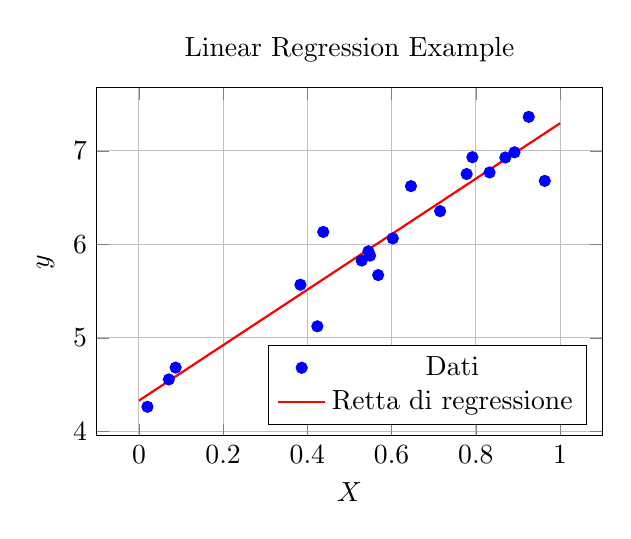
\begin{tikzpicture}
            \begin{axis}[
                width=8cm,
                height=6cm,
                xlabel={$X$},
                ylabel={$y$},
                title={Linear Regression Example},
                legend pos=south east,
                grid=major,
                ]
                % Data points
                \addplot[
                only marks,
                color=blue,
                mark=*,
                samples=100
                ] coordinates {
                    (0.5488135, 5.8798844)
                    (0.71518937, 6.3556331)
                    (0.60276338, 6.0641095)
                    (0.54488318, 5.926111)
                    (0.4236548, 5.124122)
                    (0.64589411, 6.6231887)
                    (0.43758721, 6.133222)
                    (0.891773, 6.984763)
                    (0.96366276, 6.678998)
                    (0.38344152, 5.568909)
                    (0.79172504, 6.932491)
                    (0.52889492, 5.827125)
                    (0.56804456, 5.671788)
                    (0.92559664, 7.363665)
                    (0.07103606, 4.556152)
                    (0.0871293, 4.682583)
                    (0.0202184, 4.263545)
                    (0.83261985, 6.769382)
                    (0.77815675, 6.752573)
                    (0.87001215, 6.929294)
                };
                
                % Linear regression line
                \addplot[
                color=red,
                thick
                ] coordinates {
                    (0, 4.3294)
                    (1, 1*2.9661+4.3294)
                };
                
                \legend{Dati, Retta di regressione}
            \end{axis}
        \end{tikzpicture}
        \end{minipage}%
        \hfill
        \begin{minipage}{0.4\textwidth}
            Dove $\lbrace x_i \rbrace_{i}\subset \R$ sono i dati di input e $\lbrace y_i \rbrace_{i}\subset \R$ sono i dati di output. Noi vogliamo trovare la retta $y = w\cdot x + b$ che meglio approssima i dati.
        \end{minipage}
        \end{figure}  
\end{frame}

\begin{frame}{Regressione lineare}
    \begin{figure}
        \begin{minipage}{0.65\textwidth}
    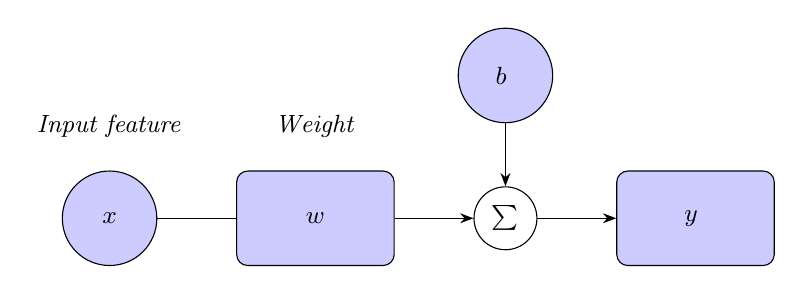
\begin{tikzpicture}
		\tikzset{
			>=Stealth,
			box/.style={draw, rounded corners, align=center, minimum height=1.2cm, minimum width=2cm, fill=blue!20},
			circlebox/.style={draw, circle, minimum size = 1.2cm, align=center, fill=blue!20},
			every node/.style={font=\small}
		}
		
		% Input nodes
		\node[circlebox] (x1) {$x$};
		
		% Weights and bias
		\node[box, right=1cm of x1] (w1) {$w$};
		
		% Sum node
		\node[draw, circle, fill=white, right=1cm of w1] (sum) { $\sum$ };
		
		% Output node
		\node[box, right=1cm of sum] (y) { $ y $ };
		
		% Bias node
		\node[circlebox, above=0.8cm of sum] (bias) { $ b $ };
		
		% Draw arrows between nodes
		\draw (x1) -- (w1);
		
		\draw[->] (w1) -- (sum);
		
		\draw[->] (bias) -- (sum);
		\draw[->] (sum) -- (y);
		
		% Annotations
		\node[above=0.3cm of w1] { \textit{Weight} };
		\node[above=0.3cm of x1] { \textit{Input feature} };
		
	\end{tikzpicture}
        \end{minipage}%
        \hfill
        \begin{minipage}{0.25\textwidth}
            \[y = w \cdot x + b\] 
            \begin{itemize}
            \item $x\in\R$ input,
            \item $w\in\R$ weight,
            \item $b\in\R$ bias.
            \end{itemize}        \end{minipage}
        \end{figure}  
\end{frame}


\begin{frame}{Regressione lineare}
    \begin{figure}
        \begin{minipage}{0.65\textwidth}
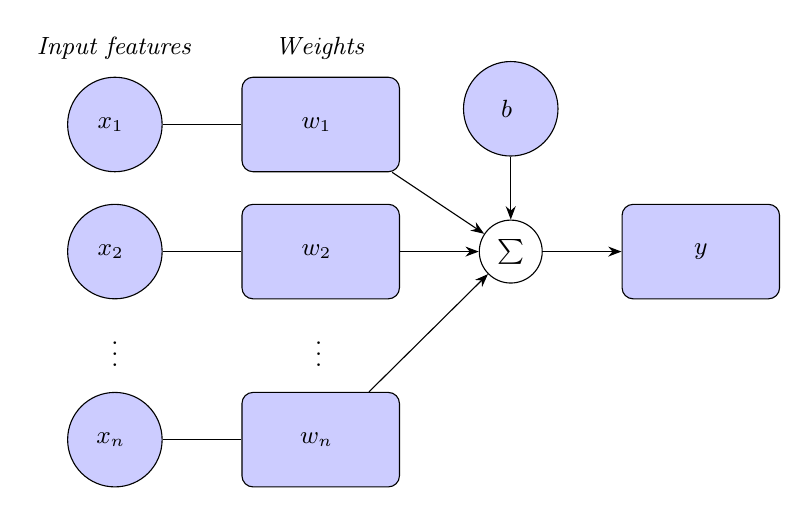
\begin{tikzpicture}
		\tikzset{
			>=Stealth,
			box/.style={draw, rounded corners, align=center, minimum height=1.2cm, minimum width=2cm, fill=blue!20},
			circlebox/.style={draw, circle, minimum size = 1.2cm, align=center, fill=blue!20},
			every node/.style={font=\small}
		}
		
		% Input nodes
		\node[circlebox] (x1) { \( x_1 \) };
		\node[circlebox, below=0.4cm of x1] (x2) { \( x_2 \) };
		\node[below=0.2cm of x2] (dots) { \vdots };
		\node[circlebox, below=0.2cm of dots] (xn) { \( x_n \) };
		
		% Weights and bias
		\node[box, right=1cm of x1] (w1) { \( w_1 \) };
		\node[box, right=1cm of x2] (w2) { \( w_2 \) };
        \node[right=2.25cm of dots] (dots_w) { \vdots };
		\node[box, right=1cm of xn] (wn) { \( w_n \) };
		
		% Sum node
		\node[draw, circle, fill=white, right=1cm of w2] (sum) { \( \sum \) };
		
		% Output node
		\node[box, right=1cm of sum] (y) {$y$};
		
		% Bias node
		\node[circlebox, above=0.8cm of sum] (bias) { \( b \) };
		
		% Draw arrows between nodes
		\draw (x1) -- (w1);
		\draw (x2) -- (w2);
		\draw (xn) -- (wn);
		
		\draw[->] (w1) -- (sum);
		\draw[->] (w2) -- (sum);
		\draw[->] (wn) -- (sum);
		
		\draw[->] (bias) -- (sum);
		\draw[->] (sum) -- (y);
		
		% Annotations
		\node[above=0.1cm of w1] { \textit{Weights} };
		\node[above=0.1cm of x1] { \textit{Input features} };
		
	\end{tikzpicture}
        \end{minipage}%
        \hfill
        \begin{minipage}{0.25\textwidth}
        \[y = \mathbf{w}\cdot \mathbf{x} + b\] 
        \begin{itemize}
        \item $\mathbf{x}\in\R^n$ inputs,
        \item $\mathbf{w}\in\R^n$ weights,
        \item $b\in\R$ bias.
        \end{itemize}
        \end{minipage}
        \end{figure}  
\end{frame}

\begin{frame}{Percettrone}
    \begin{figure}
        \begin{minipage}{0.6\textwidth}
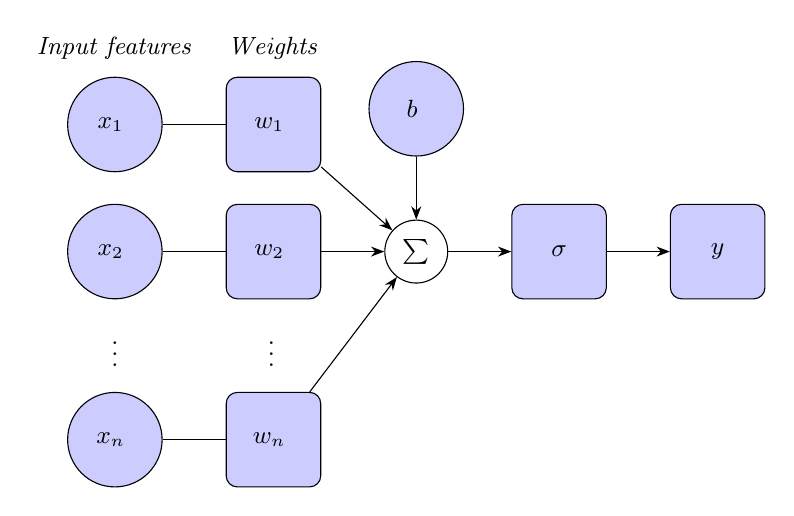
\begin{tikzpicture}
		\tikzset{
			>=Stealth,
			box/.style={draw, rounded corners, align=center, minimum height=1.2cm, minimum width=1.2cm, fill=blue!20},
			circlebox/.style={draw, circle, minimum size = 1.2cm, align=center, fill=blue!20},
			every node/.style={font=\small}
		}
		
		% Input nodes
		\node[circlebox] (x1) { \( x_1 \) };
		\node[circlebox, below=0.4cm of x1] (x2) { \( x_2 \) };
		\node[below=0.2cm of x2] (dots) { \vdots };
		\node[circlebox, below=0.2cm of dots] (xn) { \( x_n \) };
		
		% Weights and bias
		\node[box, right=0.8cm of x1] (w1) { \( w_1 \) };
		\node[box, right=0.8cm of x2] (w2) { \( w_2 \) };
        \node[right=1.65cm of dots] (dots_w) { \vdots };
		\node[box, right=0.8cm of xn] (wn) { \( w_n \) };
		
		% Sum node
		\node[draw, circle, fill=white, right=0.8cm of w2] (sum) { \( \sum \) };
		
		% activation
		\node[box, right=0.8cm of sum] (activation) {$\sigma$};

		% Output node
		\node[box, right=0.8cm of activation] (y) {$y$};
		
		% Bias node
		\node[circlebox, above=0.8cm of sum] (bias) { \( b \) };
		
		% Draw arrows between nodes
		\draw (x1) -- (w1);
		\draw (x2) -- (w2);
		\draw (xn) -- (wn);
		
		\draw[->] (w1) -- (sum);
		\draw[->] (w2) -- (sum);
		\draw[->] (wn) -- (sum);
		
		\draw[->] (bias) -- (sum);
		\draw[->] (sum) -- (activation);
        \draw[->] (activation) -- (y);
		
		% Annotations
		\node[above=0.1cm of w1] { \textit{Weights} };
		\node[above=0.1cm of x1] { \textit{Input features} };
		
	\end{tikzpicture}
        \end{minipage}%
        \hfill
        \begin{minipage}{0.3\textwidth}
        Consideriamo il problema di classificazione. 
        \[y = \sigma\left(\mathbf{w}\cdot \mathbf{x} + b\right),\] 
        con $\sigma(z) = 1$ se $z\ge 0$ e nulla altrove.
        \end{minipage}
        \end{figure}  
\end{frame}

\begin{frame}{Percettrone}
    \begin{columns}
        \begin{column}{0.5\textwidth}
            Chiamiamo $\hat{y}(\mathbf{x})$ la label corretta associata ad $\mathbf{x}$, l'algoritmo per trovare $\mathbf{w}$ e $b$ \'e:
            \begin{itemize}
                \item calcolare $y(\mathbf{x}) = \sigma\left(\mathbf{w}\cdot \mathbf{x} + b\right) $, 
                \item se $y(\mathbf{x}) = \hat{y}(\mathbf{x})$ no aggiornamento,
                \item se $y(\mathbf{x})=1 $ e $\hat{y}(\mathbf{x}) = 0$ allora aggiorniamo $\mathbf{w} = \mathbf{w} + \eta \mathbf{x}$ e $b = b + \eta$.
                \item se $y(\mathbf{x})=0 $ e $\hat{y}(\mathbf{x}) = 1$ allora aggiorniamo $\mathbf{w} = \mathbf{w} - \eta \mathbf{x}$ e $b = b - \eta$.
            \end{itemize}
        \end{column}
        \pause
        \begin{column}{0.5\textwidth}
            \begin{center}
            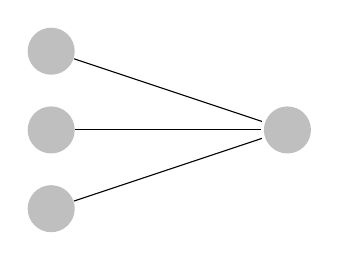
\begin{tikzpicture}[
                >=stealth,
                shorten >=1pt,
                auto,
                node distance=2cm,
                neuron/.style={circle, fill=black!25, minimum size=17pt, inner sep=0pt},
                layer/.style={thick, draw=black!50, rectangle, fill=black!10, minimum height=4em},
            ]
            
                % Draw the input layer nodes
                \foreach \name / \y in {1,...,3}
                    \node[neuron] (I-\name) at (0,-\y) {};
            
                % Draw the output layer node
                \foreach \name / \y in {2}
                    \node[neuron] (O-\name) at (3,-\y) {};
            
                % Connect every node in the input layer with every node in the
                % hidden layer.
                \foreach \source in {1,...,3}
                    \foreach \dest in {2}
                        \path (I-\source) edge (O-\dest);
            \end{tikzpicture}%
            \end{center}
            Ogni cerchio rappresenta un neurone, a cui è associato un bias. Ogni freccia rappresenta una connessione tra ue neuroni a cui è associato un peso.
        \end{column}
    \end{columns}
\end{frame}

\begin{frame}{Percettrone}
Notiamo che se $x_{0}, x_{1} \in \lbrace 0, 1 \rbrace$ allora con il percettrone si puo' rappresentare le operazioni logiche di negazione, congiunzione e disgiunzione.
\begin{figure}
    \centering
    \begin{minipage}{0.3\textwidth}
        \begin{center}
            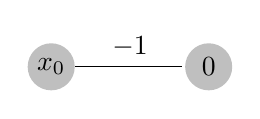
\begin{tikzpicture}[
                >=stealth,
                shorten >=1pt,
                auto,
                node distance=2cm,
                neuron/.style={circle, fill=black!25, minimum size=17pt, inner sep=0pt},
                layer/.style={thick, draw=black!50, rectangle, fill=black!10, minimum height=4em},
            ]
                % Draw the input layer nodes
                \foreach \name / \y in {0}
                    \node[neuron, align=center] (I-\name) at (0,-\y) {$x_{\y }$};

                % Draw the output layer node
                \foreach \name / \y in {0}
                    \node[neuron, align=center] (O-\name) at (2, -\y) {$0$};

                % Connect every node in the input layer with every node in the
                % hidden layer.
                \foreach \source in {0}
                    \foreach \dest in {0}
                        \path (I-\source) edge node[midway, above, sloped] {$-1$} (O-\dest);
            \end{tikzpicture}%
        \end{center}
        \caption{Negazione}
    \end{minipage}%
    \hfill
    \begin{minipage}{0.3\textwidth}
        \begin{center}
            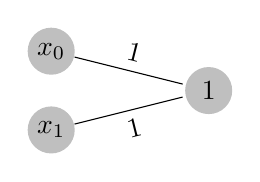
\begin{tikzpicture}[
                >=stealth,
                shorten >=1pt,
                auto,
                node distance=2cm,
                neuron/.style={circle, fill=black!25, minimum size=17pt, inner sep=0pt},
                layer/.style={thick, draw=black!50, rectangle, fill=black!10, minimum height=4em},
            ]
                % Draw the input layer nodes
                \foreach \name / \y in {0,1}
                    \node[neuron, align=center] (I-\name) at (0,-\y) {$x_{\y }$};

                % Draw the output layer node
                \foreach \name / \y in {0}
                    \node[neuron, align=center] (O-\name) at (2, -0.5-\y) {$1$};

                % Connect every node in the input layer with every node in the
                % hidden layer.
                \foreach \source in {0}
                    \foreach \dest in {0}
                        \path (I-\source) edge node[midway, above, sloped] {$1$} (O-\dest);
                \foreach \source in {1}
                    \foreach \dest in {0}
                        \path (I-\source) edge node[midway, below, sloped] {$1$} (O-\dest);
            \end{tikzpicture}%
        \end{center}
        \caption{Congiunzione}
    \end{minipage}%
    \hfill
    \begin{minipage}{0.3\textwidth}
        \begin{center}
            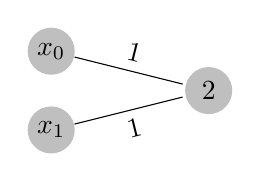
\begin{tikzpicture}[
                >=stealth,
                shorten >=1pt,
                auto,
                node distance=2cm,
                neuron/.style={circle, fill=black!25, minimum size=17pt, inner sep=0pt},
                layer/.style={thick, draw=black!50, rectangle, fill=black!10, minimum height=4em},
            ]
                % Draw the input layer nodes
                \foreach \name / \y in {0,1}
                    \node[neuron, align=center] (I-\name) at (0,-\y) {$x_{\y }$};

                % Draw the output layer node
                \foreach \name / \y in {0}
                    \node[neuron, align=center] (O-\name) at (2, -0.5-\y) {$2$};

                % Connect every node in the input layer with every node in the
                % hidden layer.
                \foreach \source in {0}
                    \foreach \dest in {0}
                        \path (I-\source) edge node[midway, above, sloped] {$1$} (O-\dest);
                \foreach \source in {1}
                    \foreach \dest in {0}
                        \path (I-\source) edge node[midway, below, sloped] {$1$} (O-\dest);
            \end{tikzpicture}%
        \end{center}
        \caption{Disgiunzione}
    \end{minipage}
\end{figure}

\pause
Ma non si puo' rappresentare la disgiunzione esclusiva (XOR).
\end{frame}

\section{Deep Learning}
\begin{frame}{Multi-layer Perceptron}
    Indicando lo XOR con $\times$ vale che
    \[
    x_{0} \times x_{1} = (x_{0} \lor x_{1}) \land \neg (x_{0} \land x_{1}) = (x_{0} \lor x_{1}) \land (\neg x_{0} \lor \neg x_{1}).
    \]
    \pause
    Dunque lo possiamo rappresentare con
    \begin{center}
        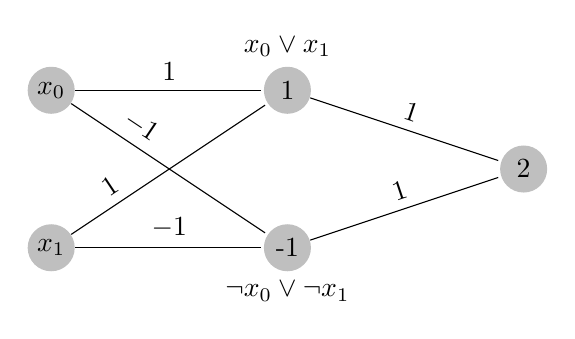
\begin{tikzpicture}[
            >=stealth,
            shorten >=1pt,
            auto,
            node distance=2cm,
            neuron/.style={circle, fill=black!25, minimum size=17pt, inner sep=0pt},
            layer/.style={thick, draw=black!50, rectangle, fill=black!10, minimum height=4em},
        ]
            % Draw the input layer nodes
            \foreach \name / \y in {0,1}
                \node[neuron, align=center] (I-\name) at (0,-2*\y) {$x_{\y}$};

            % Draw the hidden layer nodes
            \foreach \name / \y in {0}
                \node[neuron, align=center, label=above:{$x_{0} \lor x_{1}$}] (H-\name) at (3,-2*\y) {1};
            \foreach \name / \y in {1}
                \node[neuron, align=center, label=below:{$\neg x_{0} \lor \neg x_{1}$}] (H-\name) at (3,-2*\y) {-1};

            % Draw the output layer node
            \foreach \name / \y in {0}
                \node[neuron, align=center] (O-\name) at (6, -1-\y) {$2$};

            % Connect every node in the input layer with every node in the
            % hidden layer.
            \path (I-0) edge node[midway, above, sloped] {$1$} (H-0);
            \path (I-0) edge node[pos=0.3, above, sloped] {$-1$} (H-1);
            \path (I-1) edge node[pos=0.25, above, sloped] {$1$} (H-0);
            \path (I-1) edge node[midway, above, sloped] {$-1$} (H-1);

            \path (H-0) edge node[midway, above, sloped] {$1$} (O-0);
            \path (H-1) edge node[midway, above, sloped] {$1$} (O-0);
        \end{tikzpicture}%
    \end{center}
\end{frame}

\begin{frame}{Multi-layer Perceptron}
    \begin{figure}
        \begin{minipage}{0.65\textwidth}
    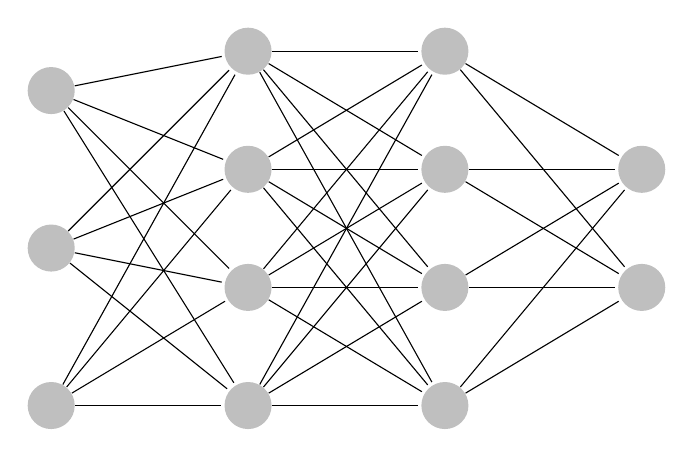
\begin{tikzpicture}[
        >=stealth,
        shorten >=1pt,
        auto,
        node distance=2cm,
        neuron/.style={circle, fill=black!25, minimum size=17pt, inner sep=0pt},
        layer/.style={thick, draw=black!50, rectangle, fill=black!10, minimum height=4em},
    ]
    
        % Draw the input layer nodes
        \foreach \name / \y in {1,...,3}
            \node[neuron] (I-\name) at (0,-\y*2) {};
    
        % Draw the hidden layer nodes
        \foreach \name / \y in {1,...,4}
            \node[neuron] (H1-\name) at (2.5,-\y*1.5) {};
            
        \foreach \name / \y in {1,...,4}
            \node[neuron] (H2-\name) at (5,-\y*1.5) {};
    
        % Draw the output layer node
        \foreach \name / \y in {2,3}
            \node[neuron] (O-\name) at (7.5,-\y*1.5) {};
    
        % Connect every node in the input layer with every node in the
        % hidden layer.
        \foreach \source in {1,...,3}
            \foreach \dest in {1,...,4}
                \path (I-\source) edge (H1-\dest);
                
        \foreach \source in {1,...,4}
            \foreach \dest in {1,...,4}
                \path (H1-\source) edge (H2-\dest);
    
        % Connect every node in the hidden layer with the output layer
        \foreach \source in {1,...,4}
            \foreach \dest in {2,3}
                \path (H2-\source) edge (O-\dest);
    \end{tikzpicture}%
        \end{minipage}%
        \hfill
        \begin{minipage}{0.35\textwidth}
        Esempio di architettura di un Multi-layer Perceptron con $3$ neuroni di input, $4$ neuroni nel primo hidden layer, $4$ neuroni nel secondo hidden layer e $2$ neuroni di output.
        \end{minipage}
        \end{figure}  
\end{frame}

\begin{frame}{Multi-layer Perceptron}
    \begin{figure}
        \begin{minipage}{0.65\textwidth}
    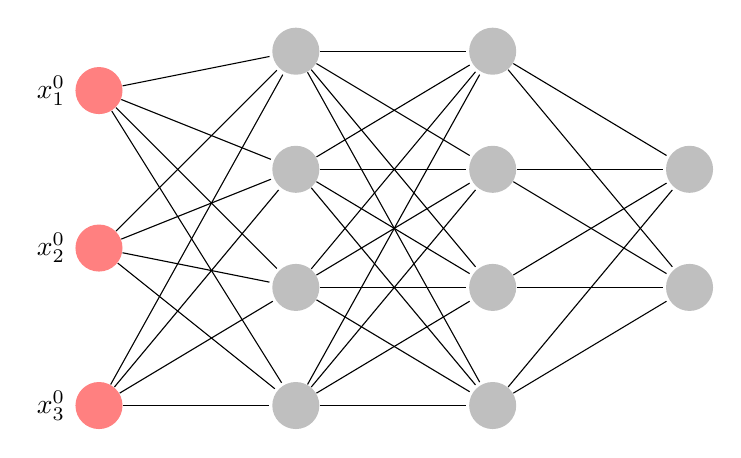
\begin{tikzpicture}[
        >=stealth,
        shorten >=1pt,
        auto,
        node distance=2cm,
        neuron/.style={circle, fill=black!25, minimum size=17pt, inner sep=0pt},
        layer/.style={thick, draw=black!50, rectangle, fill=black!10, minimum height=4em},
    ]
    
        % Draw the input layer nodes
        \foreach \name / \y in {1,...,3}
            \node[neuron, fill=red!50, label=left:{$x_{\name}^{0}$}] (I-\name) at (0,-\y*2) {};
    
        % Draw the hidden layer nodes
        \foreach \name / \y in {1,...,4}
            \node[neuron] (H1-\name) at (2.5,-\y*1.5) {};
            
        \foreach \name / \y in {1,...,4}
            \node[neuron] (H2-\name) at (5,-\y*1.5) {};
    
        % Draw the output layer node
        \foreach \name / \y in {2,3}
            \node[neuron] (O-\name) at (7.5,-\y*1.5) {};
    
        % Connect every node in the input layer with every node in the
        % hidden layer.
        \foreach \source in {1,...,3}
            \foreach \dest in {1,...,4}
                \path (I-\source) edge (H1-\dest);
                
        \foreach \source in {1,...,4}
            \foreach \dest in {1,...,4}
                \path (H1-\source) edge (H2-\dest);
    
        % Connect every node in the hidden layer with the output layer
        \foreach \source in {1,...,4}
            \foreach \dest in {2,3}
                \path (H2-\source) edge (O-\dest);
            \end{tikzpicture}%
        \end{minipage}%
        \hfill
        \begin{minipage}{0.35\textwidth}
            Layer di input con $3$ neuroni.
        \end{minipage}
        \end{figure}  
\end{frame}

\begin{frame}{Multi-layer Perceptron}
    \begin{figure}
        \begin{minipage}{0.65\textwidth}
    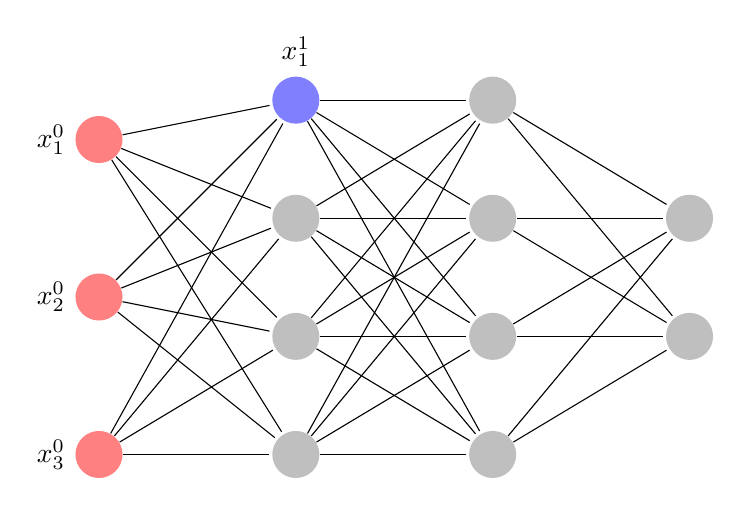
\begin{tikzpicture}[
        >=stealth,
        shorten >=1pt,
        auto,
        node distance=2cm,
        neuron/.style={circle, fill=black!25, minimum size=17pt, inner sep=0pt},
        layer/.style={thick, draw=black!50, rectangle, fill=black!10, minimum height=4em},
    ]
    
        % Draw the input layer nodes
        \foreach \name / \y in {1,...,3}
            \node[neuron, fill=red!50, label=left:{$x_{\name}^{0}$}] (I-\name) at (0,-\y*2) {};
    
        % Draw the hidden layer nodes
        \foreach \name / \y in {1}
            \node[neuron, fill=blue!50, label=above:{$x_{\name}^{1}$}] (H1-\name) at (2.5,-\y*1.5) {};
        \foreach \name / \y in {2,...,4}
            \node[neuron] (H1-\name) at (2.5,-\y*1.5) {};
            
        \foreach \name / \y in {1,...,4}
            \node[neuron] (H2-\name) at (5,-\y*1.5) {};
    
        % Draw the output layer node
        \foreach \name / \y in {2,3}
            \node[neuron] (O-\name) at (7.5,-\y*1.5) {};
    
        % Connect every node in the input layer with every node in the
        % hidden layer.
        \foreach \source in {1,...,3}
            \foreach \dest in {1,...,4}
                \path (I-\source) edge (H1-\dest);
                
        \foreach \source in {1,...,4}
            \foreach \dest in {1,...,4}
                \path (H1-\source) edge (H2-\dest);
    
        % Connect every node in the hidden layer with the output layer
        \foreach \source in {1,...,4}
            \foreach \dest in {2,3}
                \path (H2-\source) edge (O-\dest);
            \end{tikzpicture}%
        \end{minipage}%
        \hfill
        \begin{minipage}{0.35\textwidth}
        Vogliamo definire il valore del neurone $x_{1}^{1}$.
        \end{minipage}
        \end{figure}  
\end{frame}

\begin{frame}{Multi-layer Perceptron}
    \begin{figure}
        \begin{minipage}{0.65\textwidth}
    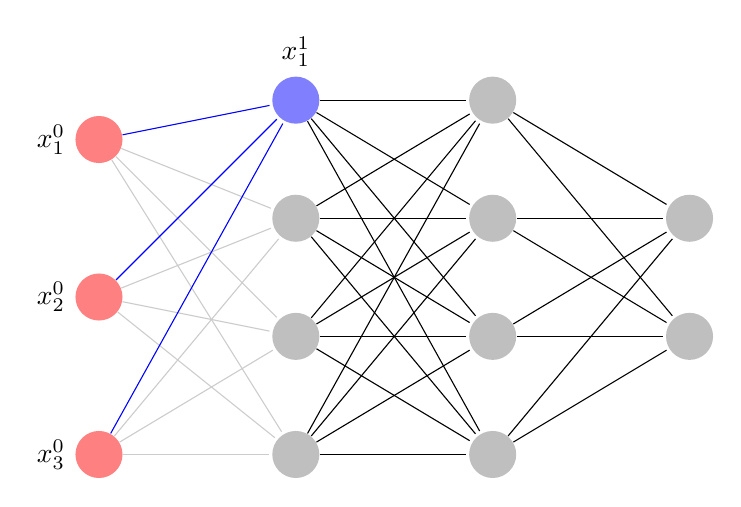
\begin{tikzpicture}[
        >=stealth,
        shorten >=1pt,
        auto,
        node distance=2cm,
        neuron/.style={circle, fill=black!25, minimum size=17pt, inner sep=0pt},
        layer/.style={thick, draw=black!50, rectangle, fill=black!10, minimum height=4em},
    ]
    
        % Draw the input layer nodes
        \foreach \name / \y in {1,...,3}
            \node[neuron, fill=red!50, label=left:{$x_{\name}^{0}$}] (I-\name) at (0,-\y*2) {};
    
        % Draw the hidden layer nodes
        \foreach \name / \y in {1}
            \node[neuron, fill=blue!50, label=above:{$x_{\name}^{1}$}] (H1-\name) at (2.5,-\y*1.5) {};
        \foreach \name / \y in {2,...,4}
            \node[neuron] (H1-\name) at (2.5,-\y*1.5) {};
            
        \foreach \name / \y in {1,...,4}
            \node[neuron] (H2-\name) at (5,-\y*1.5) {};
    
        % Draw the output layer node
        \foreach \name / \y in {2,3}
            \node[neuron] (O-\name) at (7.5,-\y*1.5) {};
    
        % Connect every node in the input layer with every node in the
        % hidden layer.
        \foreach \source in {1,...,3}
            \foreach \dest in {2, ..., 4}
                \path (I-\source) edge[draw=black!20] (H1-\dest);
        \foreach \source in {1,...,3}
            \foreach \dest in {1}
				\path (I-\source) edge[draw=blue] (H1-\dest); 
                
        \foreach \source in {1,...,4}
            \foreach \dest in {1,...,4}
                \path (H1-\source) edge (H2-\dest);
    
        % Connect every node in the hidden layer with the output layer
        \foreach \source in {1,...,4}
            \foreach \dest in {2,3}
                \path (H2-\source) edge (O-\dest);
            \end{tikzpicture}%
        \end{minipage}%
        \hfill
        \begin{minipage}{0.35\textwidth}
        Evidenziamo le connesioni con i neuroni nel layer precedente.
        \end{minipage}
        \end{figure}  
\end{frame}

\begin{frame}{Multi-layer Perceptron}
    \begin{figure}
        \begin{minipage}{0.65\textwidth}
    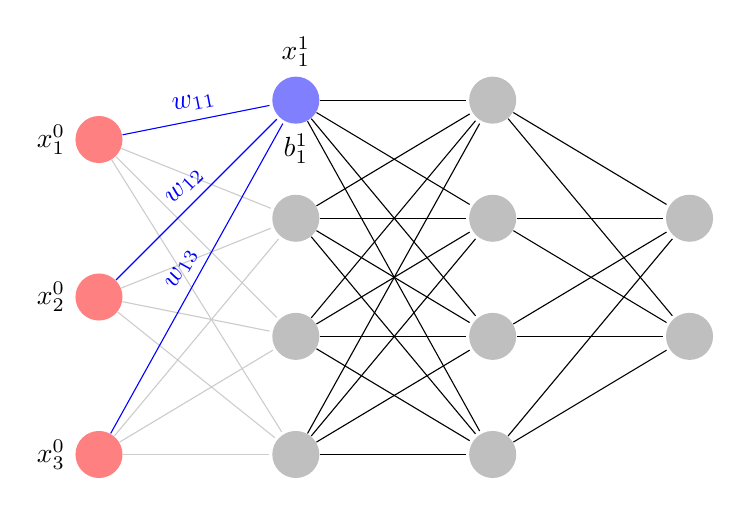
\begin{tikzpicture}[
        >=stealth,
        shorten >=1pt,
        auto,
        node distance=2cm,
        neuron/.style={circle, fill=black!25, minimum size=17pt, inner sep=0pt},
        layer/.style={thick, draw=black!50, rectangle, fill=black!10, minimum height=4em},
    ]
    
        % Draw the input layer nodes
        \foreach \name / \y in {1,...,3}
            \node[neuron, fill=red!50, label=left:{$x_{\name}^{0}$}] (I-\name) at (0,-\y*2) {};
    
        % Draw the hidden layer nodes
        \foreach \name / \y in {1}
			\node[neuron, fill=blue!50, label=above:{$x_{\name}^{1}$}, label=below:{$b_{\name}^{1}$}] (H1-\name) at (2.5,-\y*1.5) {};
        \foreach \name / \y in {2,...,4}
            \node[neuron] (H1-\name) at (2.5,-\y*1.5) {};
            
        \foreach \name / \y in {1,...,4}
            \node[neuron] (H2-\name) at (5,-\y*1.5) {};
    
        % Draw the output layer node
        \foreach \name / \y in {2,3}
            \node[neuron] (O-\name) at (7.5,-\y*1.5) {};
    
        % Connect every node in the input layer with every node in the
        % hidden layer.
        \foreach \source in {1,...,3}
            \foreach \dest in {2, ..., 4}
                \path (I-\source) edge[draw=black!20] (H1-\dest);
        \foreach \source in {1,...,3}
            \foreach \dest in {1}
				\path (I-\source) edge[draw=blue] node[midway, above, sloped, text=blue] {$w_{\dest\source}$} (H1-\dest); 
                
        \foreach \source in {1,...,4}
            \foreach \dest in {1,...,4}
                \path (H1-\source) edge (H2-\dest);
    
        % Connect every node in the hidden layer with the output layer
        \foreach \source in {1,...,4}
            \foreach \dest in {2,3}
                \path (H2-\source) edge (O-\dest);
    \end{tikzpicture}%
\end{minipage}%
\hfill
\begin{minipage}{0.35\textwidth}
    \[x_{1}^{1} = \sigma\left( b_{1}^{1} + \sum_{i=1}^{3} w_{1i}x_{i}^{0}\right)\]
    Dove $\sigma$ è una funzione di attivazione non lineare.
\end{minipage}
\end{figure}  
\end{frame}


\begin{frame}{Multi-layer Perceptron}
    \begin{figure}
        \begin{minipage}{0.65\textwidth}
    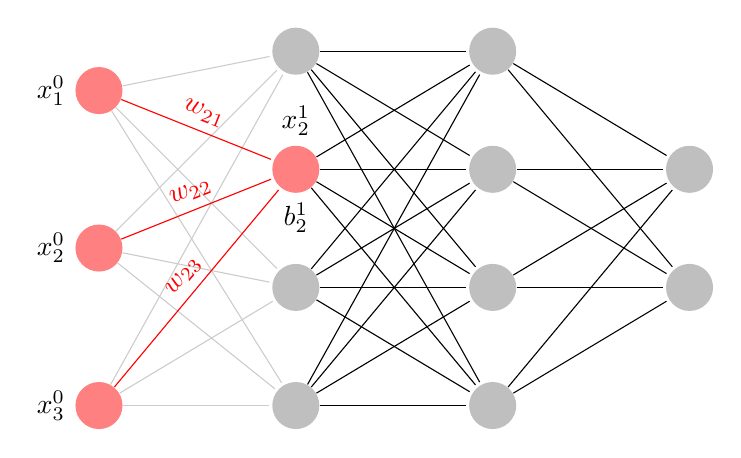
\begin{tikzpicture}[
        >=stealth,
        shorten >=1pt,
        auto,
        node distance=2cm,
        neuron/.style={circle, fill=black!25, minimum size=17pt, inner sep=0pt},
        layer/.style={thick, draw=black!50, rectangle, fill=black!10, minimum height=4em},
    ]
    
        % Draw the input layer nodes
        \foreach \name / \y in {1,...,3}
            \node[neuron, fill=red!50, label=left:{$x_{\name}^{0}$}] (I-\name) at (0,-\y*2) {};
    
        % Draw the hidden layer nodes
        \foreach \name / \y in {2}
			\node[neuron, fill=red!50, label=above:{$x_{\name}^{1}$}, label=below:{$b_{\name}^{1}$}] (H1-\name) at (2.5,-\y*1.5) {};
        \foreach \name / \y in {1, 3, 4}
            \node[neuron] (H1-\name) at (2.5,-\y*1.5) {};
            
        \foreach \name / \y in {1,...,4}
            \node[neuron] (H2-\name) at (5,-\y*1.5) {};
    
        % Draw the output layer node
        \foreach \name / \y in {2,3}
            \node[neuron] (O-\name) at (7.5,-\y*1.5) {};
    
        % Connect every node in the input layer with every node in the
        % hidden layer.
        \foreach \source in {1,...,3}
            \foreach \dest in {1, 3, 4}
                \path (I-\source) edge[draw=black!20] (H1-\dest);
        \foreach \source in {1,...,3}
            \foreach \dest in {2}
				\path (I-\source) edge[draw=red] node[midway, above, sloped, text=red] {$w_{\dest\source}$} (H1-\dest); 
                
        \foreach \source in {1,...,4}
            \foreach \dest in {1,...,4}
                \path (H1-\source) edge (H2-\dest);
    
        % Connect every node in the hidden layer with the output layer
        \foreach \source in {1,...,4}
            \foreach \dest in {2,3}
                \path (H2-\source) edge (O-\dest);
    \end{tikzpicture}%
\end{minipage}%
\hfill
\begin{minipage}{0.35\textwidth}
    \[x_{1}^{1} = \sigma\left(b_{1}^{1} +\sum_{i=1}^{3} w_{1i}x_{i}^{0} \right) \]
    \[x_{2}^{1} = \sigma\left( b_{2}^{1}+\sum_{i=1}^{4} w_{2i}x_{i}^{0} \right) \]
\end{minipage}
\end{figure}  
\end{frame}


\begin{frame}{Multi-layer Perceptron}
    \begin{figure}
        \begin{minipage}{0.65\textwidth}
    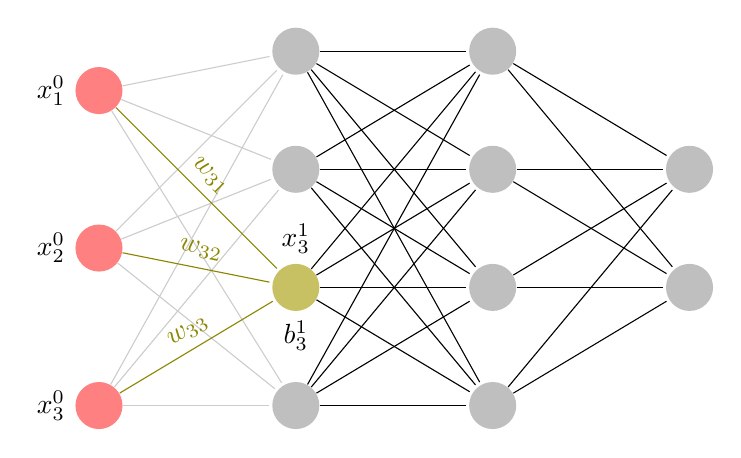
\begin{tikzpicture}[
        >=stealth,
        shorten >=1pt,
        auto,
        node distance=2cm,
        neuron/.style={circle, fill=black!25, minimum size=17pt, inner sep=0pt},
        layer/.style={thick, draw=black!50, rectangle, fill=black!10, minimum height=4em},
    ]
    
        % Draw the input layer nodes
        \foreach \name / \y in {1,...,3}
            \node[neuron, fill=red!50, label=left:{$x_{\name}^{0}$}] (I-\name) at (0,-\y*2) {};
    
        % Draw the hidden layer nodes
        \foreach \name / \y in {3}
			\node[neuron, fill=olive!50, label=above:{$x_{\name}^{1}$}, label=below:{$b_{\name}^{1}$}] (H1-\name) at (2.5,-\y*1.5) {};
        \foreach \name / \y in {1, 2, 4}
            \node[neuron] (H1-\name) at (2.5,-\y*1.5) {};
            
        \foreach \name / \y in {1,...,4}
            \node[neuron] (H2-\name) at (5,-\y*1.5) {};
    
        % Draw the output layer node
        \foreach \name / \y in {2,3}
            \node[neuron] (O-\name) at (7.5,-\y*1.5) {};
    
        % Connect every node in the input layer with every node in the
        % hidden layer.
        \foreach \source in {1,...,3}
            \foreach \dest in {1, 2, 4}
                \path (I-\source) edge[draw=black!20] (H1-\dest);
        \foreach \source in {1,...,3}
            \foreach \dest in {3}
				\path (I-\source) edge[draw=olive] node[midway, above, sloped, text=olive] {$w_{\dest\source}$} (H1-\dest); 
                
        \foreach \source in {1,...,4}
            \foreach \dest in {1,...,4}
                \path (H1-\source) edge (H2-\dest);
    
        % Connect every node in the hidden layer with the output layer
        \foreach \source in {1,...,4}
            \foreach \dest in {2,3}
                \path (H2-\source) edge (O-\dest);
    \end{tikzpicture}%
\end{minipage}%
\hfill
\begin{minipage}{0.35\textwidth}
    \[x_{1}^{1} = \sigma\left(b_{1}^{1}+\sum_{i=1}^{3} w_{1i}x_{i}^{0} \right) \]
    \[x_{2}^{1} = \sigma\left(b_{2}^{1}+\sum_{i=1}^{4} w_{2i}x_{i}^{0} \right) \]
    \[x_{3}^{1} = \sigma\left(b_{3}^{1}+\sum_{i=1}^{4} w_{3i}x_{i}^{0} \right) \]
\end{minipage}
\end{figure}  
\end{frame}


\begin{frame}{Multi-layer Perceptron}
    \begin{figure}
        \begin{minipage}{0.65\textwidth}
    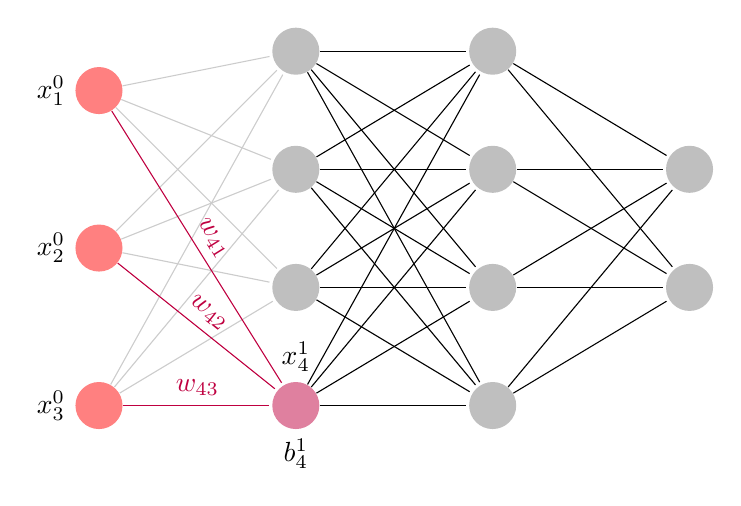
\begin{tikzpicture}[
        >=stealth,
        shorten >=1pt,
        auto,
        node distance=2cm,
        neuron/.style={circle, fill=black!25, minimum size=17pt, inner sep=0pt},
        layer/.style={thick, draw=black!50, rectangle, fill=black!10, minimum height=4em},
    ]
    
        % Draw the input layer nodes
        \foreach \name / \y in {1,...,3}
            \node[neuron, fill=red!50, label=left:{$x_{\name}^{0}$}] (I-\name) at (0,-\y*2) {};
    
        % Draw the hidden layer nodes
        \foreach \name / \y in {4}
			\node[neuron, fill=purple!50, label=above:{$x_{\name}^{1}$}, label=below:{$b_{\name}^{1}$}] (H1-\name) at (2.5,-\y*1.5) {};
        \foreach \name / \y in {1, ..., 3}
            \node[neuron] (H1-\name) at (2.5,-\y*1.5) {};
            
        \foreach \name / \y in {1,...,4}
            \node[neuron] (H2-\name) at (5,-\y*1.5) {};
    
        % Draw the output layer node
        \foreach \name / \y in {2,3}
            \node[neuron] (O-\name) at (7.5,-\y*1.5) {};
    
        % Connect every node in the input layer with every node in the
        % hidden layer.
        \foreach \source in {1,...,3}
            \foreach \dest in {1, ..., 3}
                \path (I-\source) edge[draw=black!20] (H1-\dest);
        \foreach \source in {1,...,3}
            \foreach \dest in {4}
				\path (I-\source) edge[draw=purple] node[midway, above, sloped, text=purple] {$w_{\dest\source}$} (H1-\dest); 
                
        \foreach \source in {1,...,4}
            \foreach \dest in {1,...,4}
                \path (H1-\source) edge (H2-\dest);
    
        % Connect every node in the hidden layer with the output layer
        \foreach \source in {1,...,4}
            \foreach \dest in {2,3}
                \path (H2-\source) edge (O-\dest);
    \end{tikzpicture}%
\end{minipage}%
\hfill
\begin{minipage}{0.35\textwidth}
    \vspace{-1cm}
    \[x_{1}^{1} = \sigma\left(b_{1}^{1}+\sum_{i=1}^{3} w_{1i}x_{i}^{0} \right) \]
    \[x_{2}^{1} = \sigma\left(b_{2}^{1}+\sum_{i=1}^{4} w_{2i}x_{i}^{0} \right) \]
    \[x_{3}^{1} = \sigma\left(b_{3}^{1}+\sum_{i=1}^{4} w_{3i}x_{i}^{0} \right) \]
    \[x_{4}^{1} = \sigma\left(b_{4}^{1}+\sum_{i=1}^{2} w_{4i}x_{i}^{0} \right) \]
\end{minipage}
\end{figure}  
\end{frame}


\begin{frame}{Multi-layer Perceptron}
    \begin{figure}
        \begin{minipage}{0.65\textwidth}
    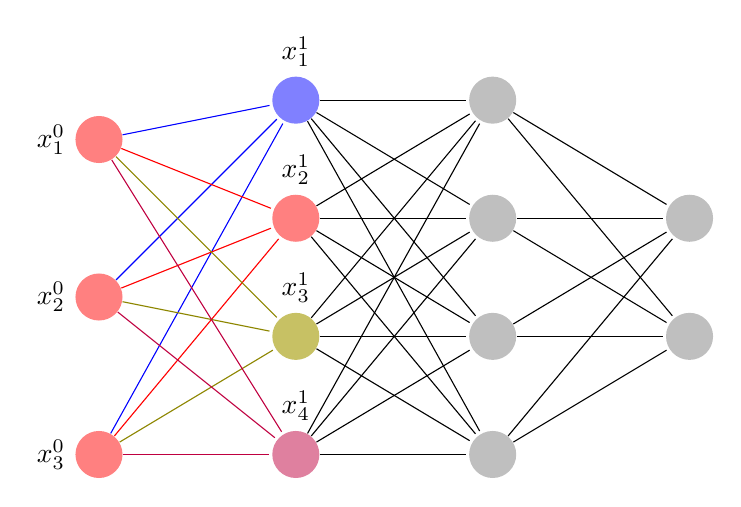
\begin{tikzpicture}[
        >=stealth,
        shorten >=1pt,
        auto,
        node distance=2cm,
        neuron/.style={circle, fill=black!25, minimum size=17pt, inner sep=0pt},
        layer/.style={thick, draw=black!50, rectangle, fill=black!10, minimum height=4em},
    ]
    
        % Draw the input layer nodes
        \foreach \name / \y in {1,...,3}
            \node[neuron, fill=red!50, label=left:{$x_{\name}^{0}$}] (I-\name) at (0,-\y*2) {};
    
        % Draw the hidden layer nodes
        \foreach \name / \y in {1}
			\node[neuron, fill=blue!50, label=above:{$x_{\name}^{1}$}] (H1-\name) at (2.5,-\y*1.5) {};
        \foreach \name / \y in {2}
			\node[neuron, fill=red!50, label=above:{$x_{\name}^{1}$}] (H1-\name) at (2.5,-\y*1.5) {};
        \foreach \name / \y in {3}
			\node[neuron, fill=olive!50, label=above:{$x_{\name}^{1}$}] (H1-\name) at (2.5,-\y*1.5) {};
        \foreach \name / \y in {4}
			\node[neuron, fill=purple!50, label=above:{$x_{\name}^{1}$}] (H1-\name) at (2.5,-\y*1.5) {};
            
        \foreach \name / \y in {1,...,4}
            \node[neuron] (H2-\name) at (5,-\y*1.5) {};
    
        % Draw the output layer node
        \foreach \name / \y in {2,3}
            \node[neuron] (O-\name) at (7.5,-\y*1.5) {};
    
        % Connect every node in the input layer with every node in the
        % hidden layer.
        \foreach \source in {1,...,3}
            \foreach \dest in {1}
				\path (I-\source) edge[draw=blue]  (H1-\dest); 
        \foreach \source in {1,...,3}
            \foreach \dest in {2}
				\path (I-\source) edge[draw=red] (H1-\dest); 
        \foreach \source in {1,...,3}
            \foreach \dest in {3}
				\path (I-\source) edge[draw=olive] (H1-\dest); 
        \foreach \source in {1,...,3}
            \foreach \dest in {4}
				\path (I-\source) edge[draw=purple]  (H1-\dest); 
                
        \foreach \source in {1,...,4}
            \foreach \dest in {1,...,4}
                \path (H1-\source) edge (H2-\dest);
    
        % Connect every node in the hidden layer with the output layer
        \foreach \source in {1,...,4}
            \foreach \dest in {2,3}
                \path (H2-\source) edge (O-\dest);
    \end{tikzpicture}%
\end{minipage}%
\hfill
\begin{minipage}{0.35\textwidth}
    Dato $\mathbf{x}^{0} \in \R^{3}$
    \[
    \mathbf{x}^{1} := \sigma\left( \mathbf{W}_{1} \mathbf{x}^{0} + \mathbf{b}_{1} \right) \in \R^{4}
    \]
    con $\mathbf{W}\in \R^{4\times 3}$, $\mathbf{b}\in \R^{4}$ e $\sigma$ funzione di attivazione non lineare applicata componente per componente.
\end{minipage}
\end{figure}  
\end{frame}


\begin{frame}{Multi-layer Perceptron}
    \begin{figure}
        \begin{minipage}{0.65\textwidth}
    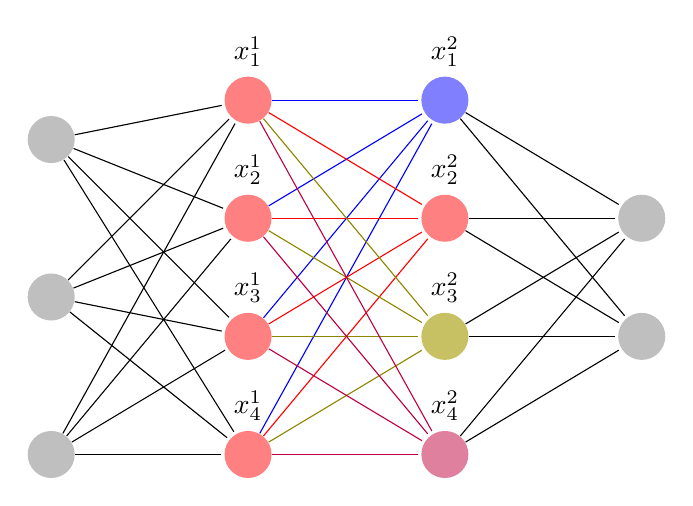
\begin{tikzpicture}[
        >=stealth,
        shorten >=1pt,
        auto,
        node distance=2cm,
        neuron/.style={circle, fill=black!25, minimum size=17pt, inner sep=0pt},
        layer/.style={thick, draw=black!50, rectangle, fill=black!10, minimum height=4em},
    ]
    
        % Draw the input layer nodes
        \foreach \name / \y in {1,...,3}
            \node[neuron] (I-\name) at (0,-\y*2) {};
    
        % Draw the hidden layer nodes
        \foreach \name / \y in {1, ..., 4}
			\node[neuron, fill=red!50, label=above:{$x_{\name}^{1}$}] (H1-\name) at (2.5,-\y*1.5) {};
            
        \foreach \name / \y in {1}
			\node[neuron, fill=blue!50, label=above:{$x_{\name}^{2}$}] (H2-\name) at (5,-\y*1.5) {};
        \foreach \name / \y in {2}
			\node[neuron, fill=red!50, label=above:{$x_{\name}^{2}$}] (H2-\name) at (5,-\y*1.5) {};
        \foreach \name / \y in {3}
			\node[neuron, fill=olive!50, label=above:{$x_{\name}^{2}$}] (H2-\name) at (5,-\y*1.5) {};
        \foreach \name / \y in {4}
			\node[neuron, fill=purple!50, label=above:{$x_{\name}^{2}$}] (H2-\name) at (5,-\y*1.5) {};
    
        % Draw the output layer node
        \foreach \name / \y in {2,3}
            \node[neuron] (O-\name) at (7.5,-\y*1.5) {};
    
        % Connect every node in the input layer with every node in the
        % hidden layer.
        \foreach \source in {1,...,3}
            \foreach \dest in {1,...,4}
                \path (I-\source) edge (H1-\dest);
    
        \foreach \source in {1,...,4}
            \foreach \dest in {1}
				\path (H1-\source) edge[draw=blue] (H2-\dest); 
        \foreach \source in {1,...,4}
            \foreach \dest in {2}
				\path (H1-\source) edge[draw=red] (H2-\dest); 
        \foreach \source in {1,...,4}
            \foreach \dest in {3}
				\path (H1-\source) edge[draw=olive] (H2-\dest); 
        \foreach \source in {1,...,4}
            \foreach \dest in {4}
				\path (H1-\source) edge[draw=purple] (H2-\dest); 
                
        % Connect every node in the hidden layer with the output layer
        \foreach \source in {1,...,4}
            \foreach \dest in {2,3}
                \path (H2-\source) edge (O-\dest);
    \end{tikzpicture}%
\end{minipage}%
\hfill
\begin{minipage}{0.35\textwidth}
    Dato $\mathbf{x}^{0} \in \R^{3}$
    \[
    \mathbf{x}^{1} := \sigma\left( \mathbf{W}_{1} \mathbf{x}^{0} + \mathbf{b}_{1} \right) \in \R^{4}
    \]
    \[
    \mathbf{x}^{2} := \sigma\left( \mathbf{W}_{2} \mathbf{x}^{1} + \mathbf{b}_{2} \right) \in \R^{4}
    \]
    con $\mathbf{W}_{2} \in \R^{4\times 4}$ e $\mathbf{b}\in \R^{4}$.
\end{minipage}
\end{figure}  
\end{frame}


\begin{frame}{Multi-layer Perceptron}
    \begin{figure}
        \begin{minipage}{0.65\textwidth}
    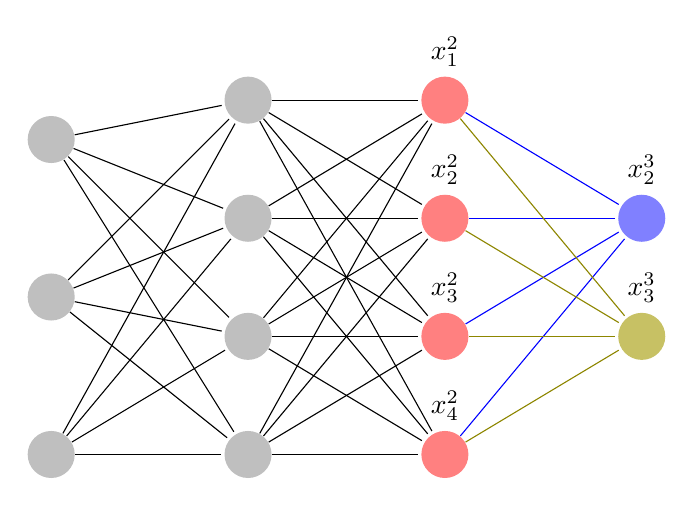
\begin{tikzpicture}[
        >=stealth,
        shorten >=1pt,
        auto,
        node distance=2cm,
        neuron/.style={circle, fill=black!25, minimum size=17pt, inner sep=0pt},
        layer/.style={thick, draw=black!50, rectangle, fill=black!10, minimum height=4em},
    ]
    
        % Draw the input layer nodes
        \foreach \name / \y in {1,...,3}
            \node[neuron] (I-\name) at (0,-\y*2) {};
    
        % Draw the hidden layer nodes
        \foreach \name / \y in {1, ..., 4}
			\node[neuron] (H1-\name) at (2.5,-\y*1.5) {};
            
        \foreach \name / \y in {1, ..., 4}
			\node[neuron, fill=red!50, label=above:{$x_{\name}^{2}$}] (H2-\name) at (5,-\y*1.5) {};
    
        % Draw the output layer node
        \foreach \name / \y in {2}
			\node[neuron, fill=blue!50, label=above:{$x_{\name}^{3}$}] (O-\name) at (7.5,-\y*1.5) {};
        \foreach \name / \y in {3}
			\node[neuron, fill=olive!50, label=above:{$x_{\name}^{3}$}] (O-\name) at (7.5,-\y*1.5) {};
    
        % Connect every node in the input layer with every node in the
        % hidden layer.
        \foreach \source in {1,...,3}
            \foreach \dest in {1,...,4}
                \path (I-\source) edge (H1-\dest);
    
        \foreach \source in {1,...,4}
            \foreach \dest in {1,...,4}
                \path (H1-\source) edge (H2-\dest);
                
        % Connect every node in the hidden layer with the output layer
        \foreach \source in {1,...,4}
            \foreach \dest in {2}
				\path (H2-\source) edge[draw=blue] (O-\dest); 
        \foreach \source in {1,...,4}
            \foreach \dest in {3}
				\path (H2-\source) edge[draw=olive] (O-\dest); 
    \end{tikzpicture}%
\end{minipage}%
\hfill
\begin{minipage}{0.35\textwidth}
    Dato $\mathbf{x}^{0} \in \R^{3}$
    \[
    \mathbf{x}^{1} := \sigma\left( \mathbf{W}_{1} \mathbf{x}^{0} + \mathbf{b}_{1} \right) \in \R^{4}
    \]
    \[
    \mathbf{x}^{2} := \sigma\left( \mathbf{W}_{2} \mathbf{x}^{1} + \mathbf{b}_{2} \right) \in \R^{4}
    \]
    \[
    \mathbf{x}^{3} := \sigma\left( \mathbf{W}_{3} \mathbf{x}^{2} + \mathbf{b}_{3} \right) \in \R^{2}
    \]
    con $\mathbf{W}_{3}\in \R^{2\times 4}$ e $\mathbf{b}\in \R^{2}$.
\end{minipage}
\end{figure}  
\end{frame}

\begin{frame}{Multi-layer Perceptron}
 \begin{definition}
  Un Multi-layer Perceptron (MLP) con input $\mathbf{x}^{0}\in \R^{d_{0}}$, $L$ hidden layers con $d_{1}, \ldots, d_{L}$ neuroni e output $\mathbf{x}^{L}\in \R^{d_{L}}$ è definito come
    \begin{align*}
     \mathbf{x}^{1} &:= \sigma\left( \mathbf{W}_{1} \mathbf{x}^{0} + \mathbf{b}_{1} \right) \in \R^{d_{1}} \\
     &\vdots \\
     \mathbf{x}^{L} &:= \sigma\left( \mathbf{W}_{L} \mathbf{x}^{L-1} + \mathbf{b}_{L} \right) \in \R^{d_{L}}
    \end{align*}
    dove $\mathbf{W}_{\ell}\in \R^{d_{\ell}\times d_{\ell-1}}$ e $\mathbf{b}_{\ell}\in \R^{d_{\ell}}$ per $\ell=1,\ldots, L$ e $\sigma$ è una funzione di attivazione non lineare applicata componente per componente.
 \end{definition}
\end{frame}

\begin{frame}{Metodo del gradiente}
    \begin{columns}[T] % align columns
        \begin{column}{.65\textwidth}
    Definito un MLP e scelta una funzione di costo $C(\mathbf{x}, \mathbf{y})$ con $\mathbf{y}$ target, si vuole minimizzare $C$ rispetto ai parametri $\mathbf{W}_{\ell}$ e $\mathbf{b}_{\ell}$. 
    \begin{definition}
        Il metodo del gradiente è un metodo iterativo per minimizzare una funzione $MLP(\mathbf{p})$ definita su uno spazio $\R^{d}$. Dato un punto iniziale $\mathbf{p}^{(0)}$, la sequenza $\mathbf{p}^{(t)}$ è definita come   
        \[
        \mathbf{p}^{(t+1)} = \mathbf{p}^{(t)} - \eta \nabla f(\mathbf{p}^{(t)})
        \]
        dove $\eta$ è il learning rate.
    \end{definition}
\end{column}%
\pause
\begin{column}[T]{.35\textwidth}
    \begin{figure}
        \centering
        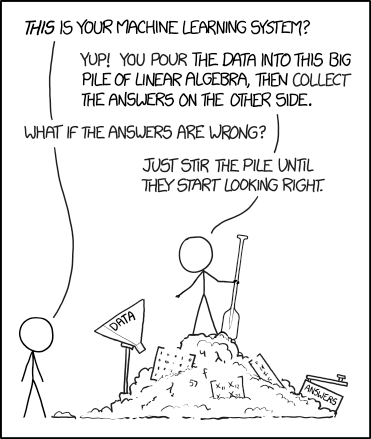
\includegraphics[height = 0.6\textheight]{memes/meme1.png}
    \end{figure}
\end{column}
\end{columns}
\end{frame}

\begin{frame}{Approsimazione universale per funzioni}
    \begin{definition}
        Una funzione continua $f: \R \to \R$ si dice sigmoidale se 
        \[ \lim_{x \to -\infty} f(x) = 0  \quad \text{e} \quad  \lim_{x \to +\infty} f(x) = 1. \]
    \end{definition}
    \pause
    \begin{theorem}
        Sia $K \subset \R^{d}$ chiuso e limitato e con $d \in \N$ e $\sigma: \R \to \R$ funzione sigmoidale allora $MLP(\sigma, d, 2)$ \'e denso in $C(K)$.
    
    \end{theorem}
    Questo significa che per ogni $f \in C(K)$ e $\varepsilon > 0$ esiste una rete neurale $f_{\theta} \in MLP(\sigma, d, 2)$ tale che $\|f - f_{\theta}\|_{\infty} < \varepsilon$.
\end{frame}

\begin{frame}{Convolutional Neural Network (CNN)}
\begin{figure}
    \begin{minipage}{0.7\textwidth}
        \centering
        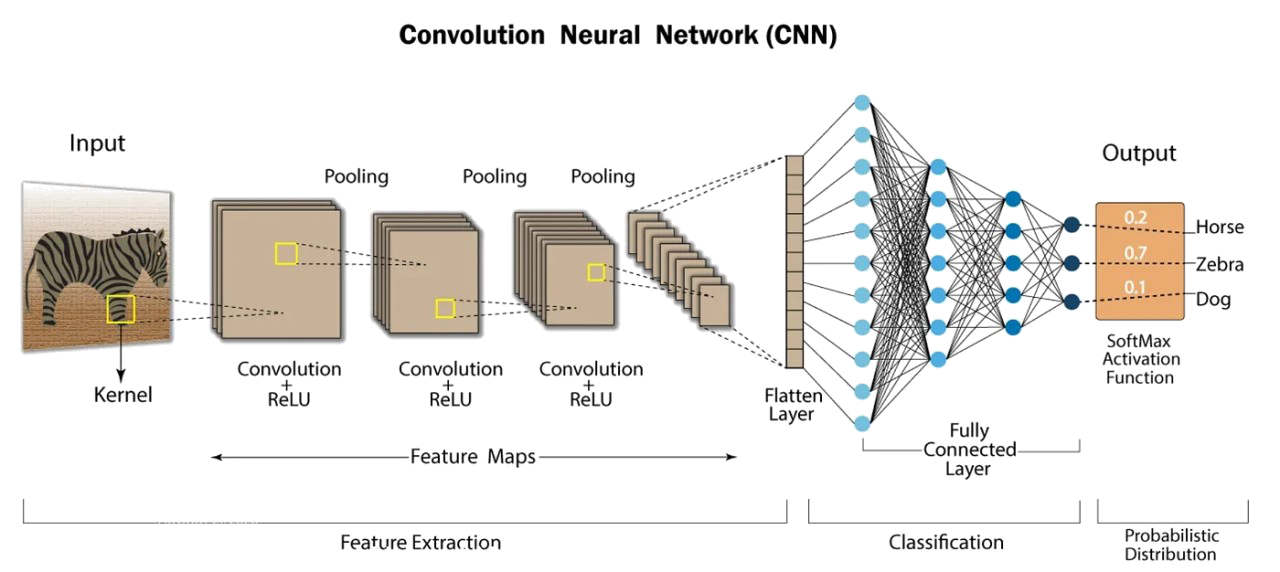
\includegraphics[width=\textwidth]{architectures/CNN.png}
    \end{minipage}%
    \begin{minipage}{0.3\textwidth}
        \centering
        Reti neurali convoluzionali per l'applicazione alle immagini.
    \end{minipage}
\end{figure}
\end{frame}

\begin{frame}{Recurrent Neural Network (RNN)}
    \begin{figure}
        \begin{minipage}{0.7\textwidth}
            \centering
            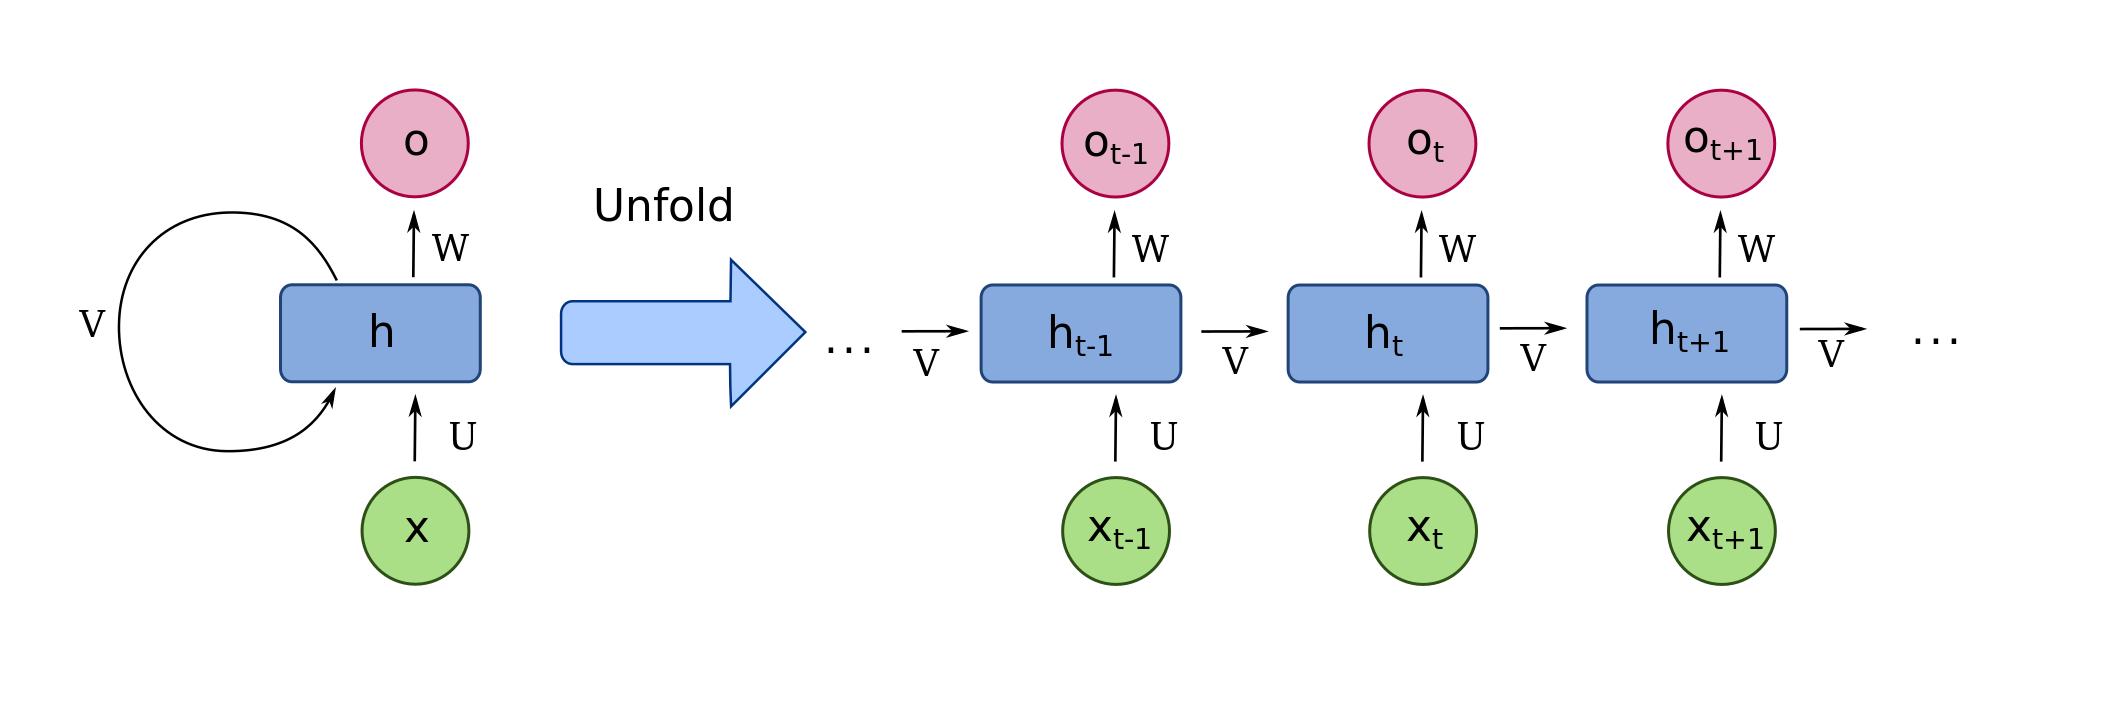
\includegraphics[width=\textwidth]{architectures/RNN.png}
        \end{minipage}%
        \begin{minipage}{0.3\textwidth}
            \centering
            Reti neurali ricorrenti per l'applicazione al linguaggio naturale ed ai segnali, o pi\'u in generale alle quantit\'a dipendenti dal tempo.
        \end{minipage}
    \end{figure}
\end{frame}

\begin{frame}{Transformer}
    \begin{figure}
        \begin{minipage}[T]{0.5\textwidth}
            \centering
            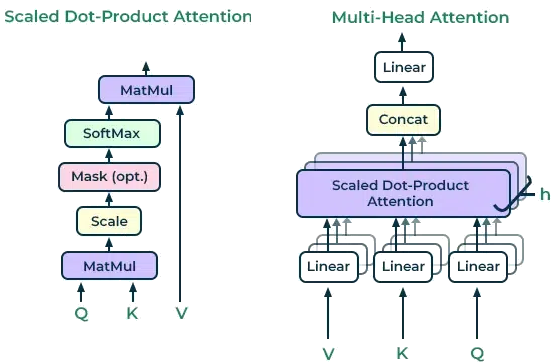
\includegraphics[height=0.6\textheight]{architectures/attention.png}
        \end{minipage}%
        \hfill
        \begin{minipage}[T]{0.35\textwidth}
            \centering
            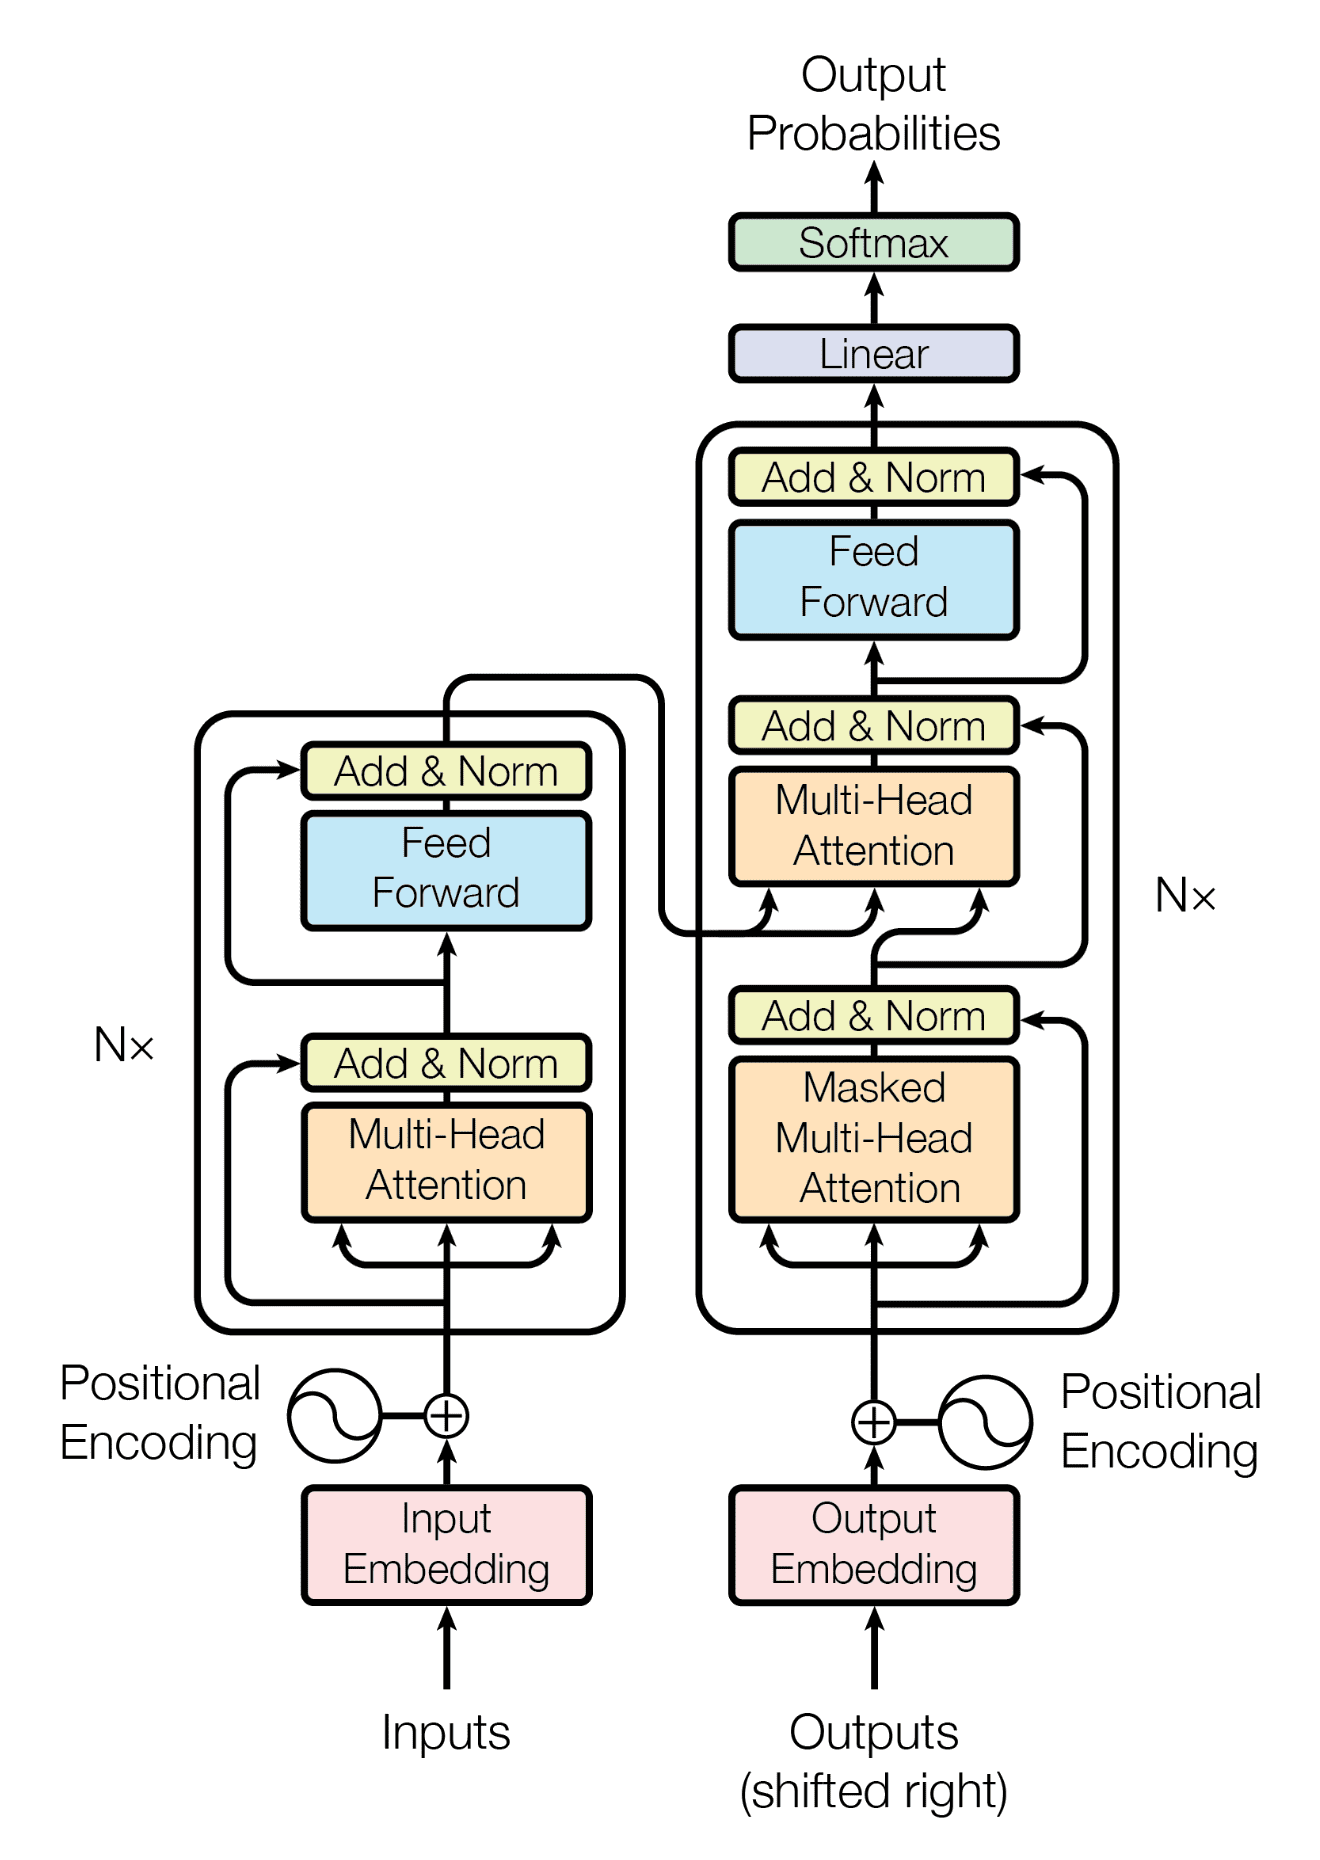
\includegraphics[height=0.8\textheight]{architectures/transformer.png}
        \end{minipage}
        \caption*{From "Attention is All You Need", Vaswani et al. (2017)}
    \end{figure}
    % \footnotetext*{"Attention is All You Need", Vaswani et al. (2017)}
\end{frame}

\section{Applicazioni interessanti}


\begin{frame}{Applicazioni alle immagini}
    Siti per generazione d'immagini: \href{https://openai.com/index/dall-e-3/}{DALL-E3} \adjustbox{valign=m}{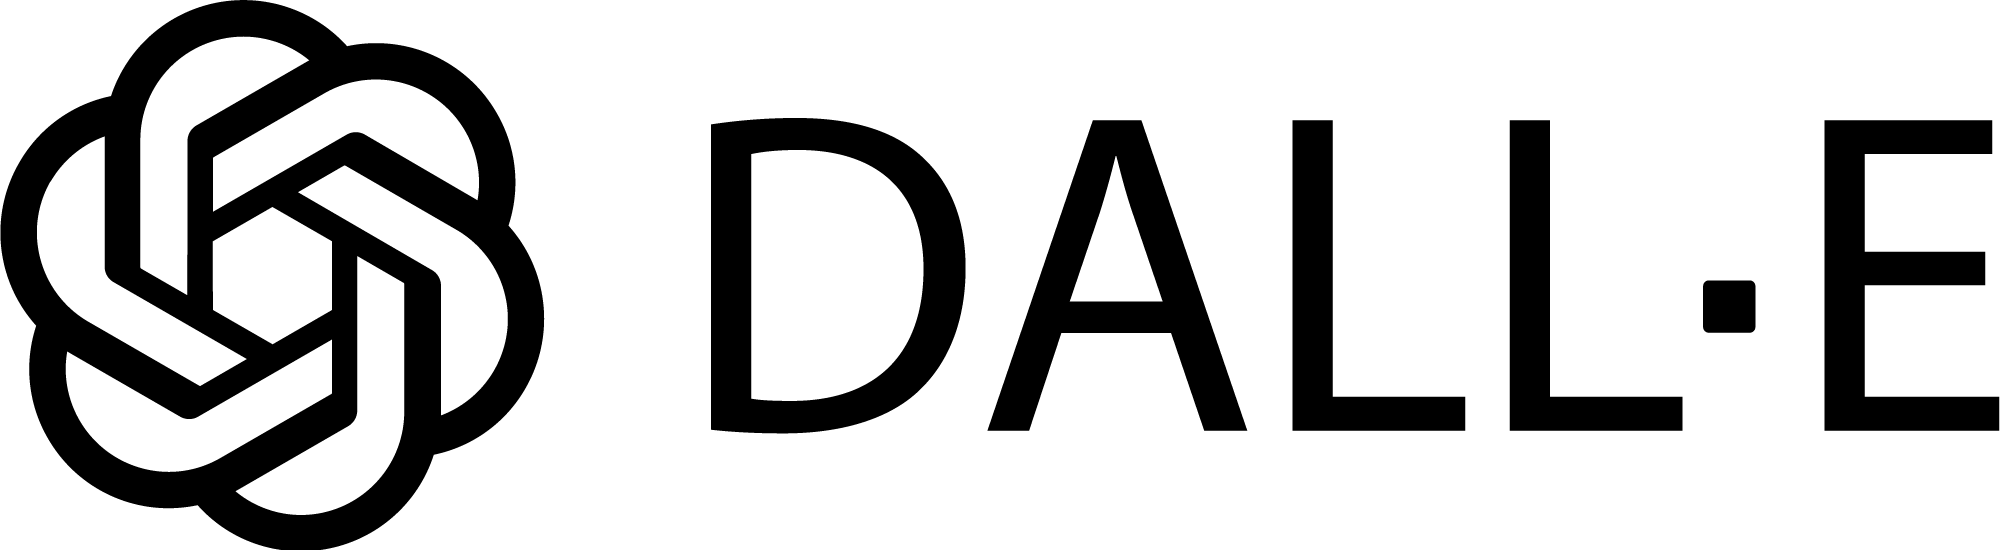
\includegraphics[width=1.5cm]{logos/logo-dall-e.png}}, \href{https://www.midjourney.com/home}{Midjourney}  \adjustbox{valign=m}{
\includegraphics[width=0.5cm]{logos/logo-midjourney.png}} e \href{https://ideogram.ai/t/top/1}{Ideogram} \adjustbox{valign=m}{
\includegraphics[width=0.5cm]{logos/logo-ideogram.png}}.
        \begin{center}
            \begin{minipage}{0.23\textwidth}
                
\includegraphics[height=0.7\textheight, width=\textwidth]{AIimages/ideogram1.png}
            \end{minipage}%
            \hfill
            \begin{minipage}{0.23\textwidth}
                
\includegraphics[height=0.7\textheight, width=\textwidth]{AIimages/ideogram2.png}
            \end{minipage}%
            \hfill
            \begin{minipage}{0.23\textwidth}
                
\includegraphics[height=0.7\textheight, width=\textwidth]{AIimages/ideogram4.jpg}
            \end{minipage}%
            \hfill
            \begin{minipage}{0.23\textwidth}
                
\includegraphics[height=0.7\textheight, width=\textwidth]{AIimages/ideogram3.png}
            \end{minipage}
        \end{center}
\end{frame}

\begin{frame}{Applicazioni ai video}
    Deep learning per la generazione di video \href{https://openai.com/index/sora/}{SORA} \adjustbox{valign=m}{
\includegraphics[width=1.5cm]{logos/logo-sora.png}} o per modificare video anche in tempo reale \href{https://www.nvidia.com/it-it/geforce/broadcasting/broadcast-app/}{NVIDIA Broadcast} \adjustbox{valign=m}{
\includegraphics[width=0.5cm]{logos/logo-broadcast.png}}.
    \vspace{-0.6cm}
    \begin{columns}[T] % align columns
        \begin{column}{.33\textwidth}
            \begin{center}
                % \includemovie[autostart,loop,poster]{0.8\textwidth}{0.7\textheight}{sora1.mp4}
                \movie[externalviewer]{
\includegraphics[width=0.8\textwidth]{videos/sora1-img.png}}{videos/sora1.mp4}
            \end{center}
        \end{column}%
        \begin{column}{.33\textwidth}
            \begin{center}
                % \includemovie[autostart,loop,poster]{0.8\textwidth}{0.7\textheight}{sora2.mp4}
                \movie[externalviewer]{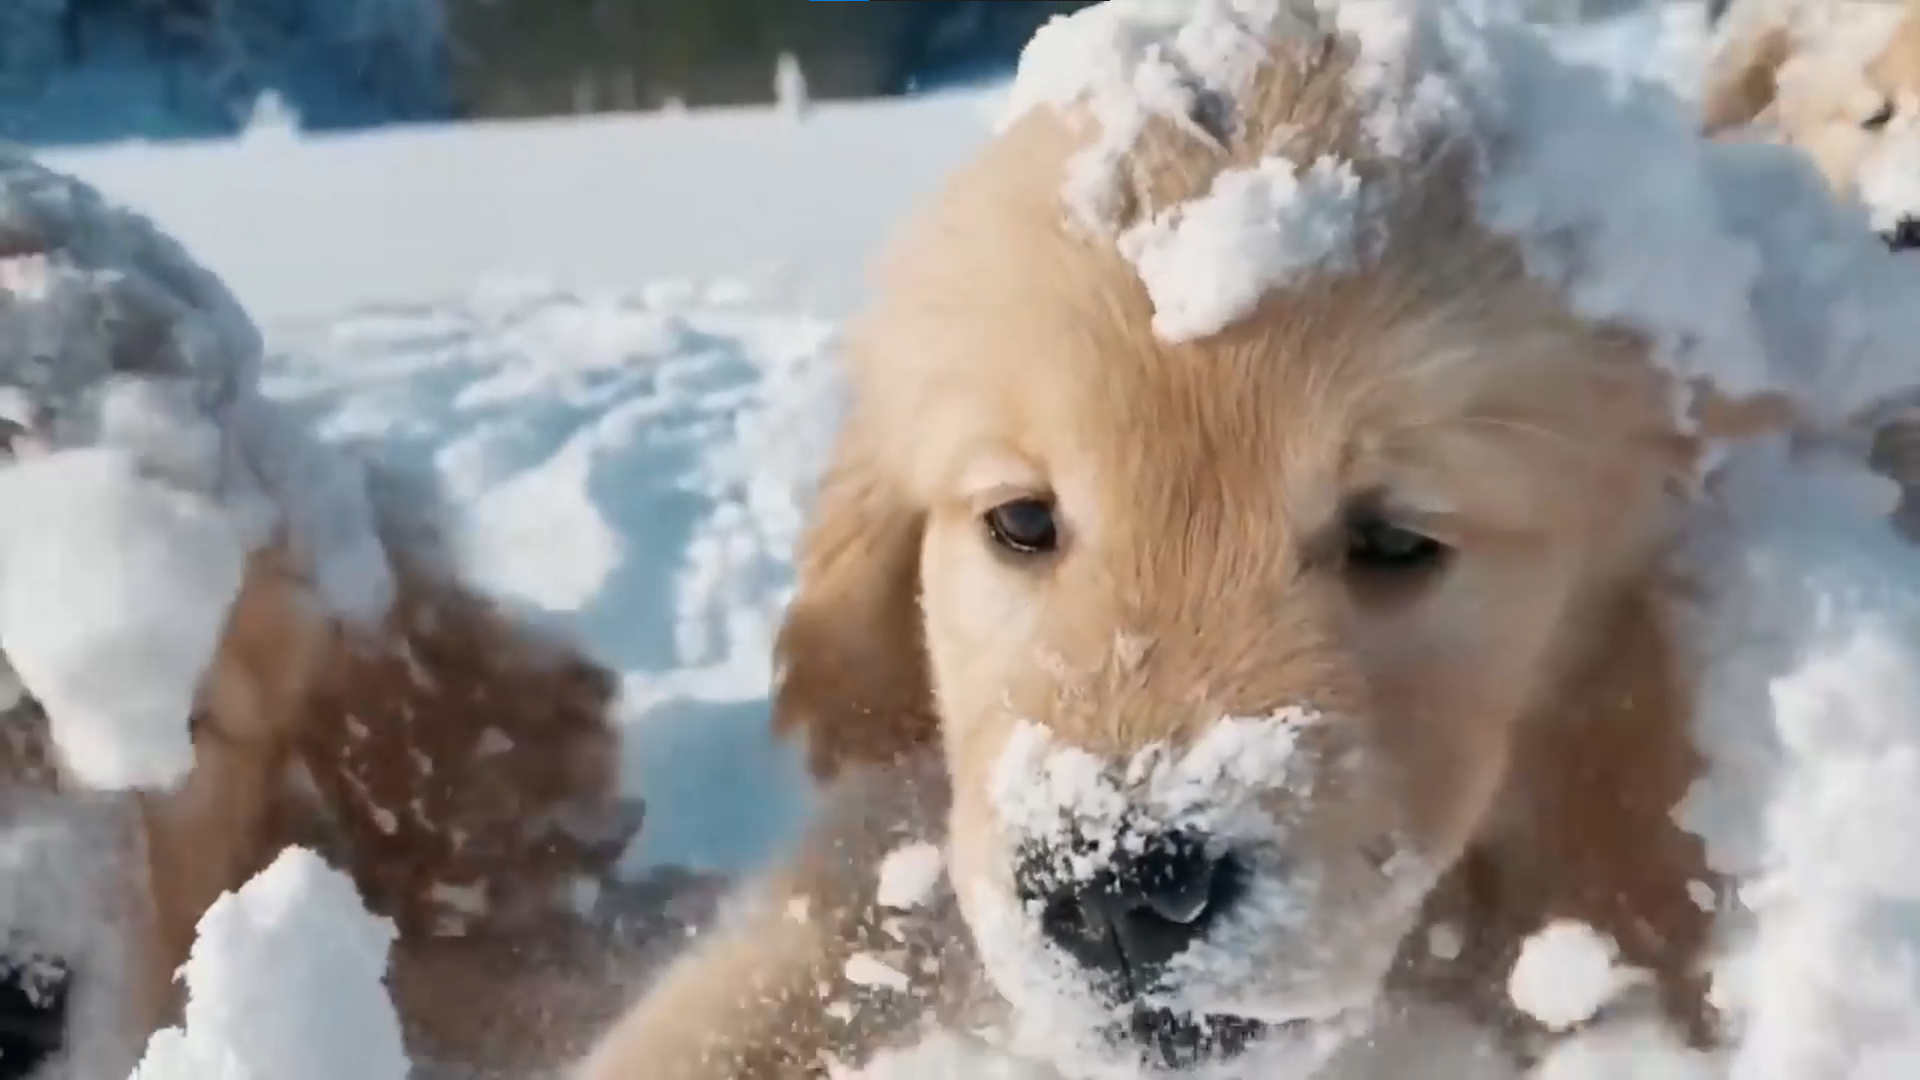
\includegraphics[width=0.8\textwidth]{videos/sora2-img.png}}{videos/sora2.mp4}
            \end{center}
        \end{column}%
        \begin{column}{.33\textwidth}
            \begin{center}
                % \includemovie[autostart,loop,poster]{0.8\textwidth}{0.7\textheight}{sora5.mp4}
                \movie[externalviewer]{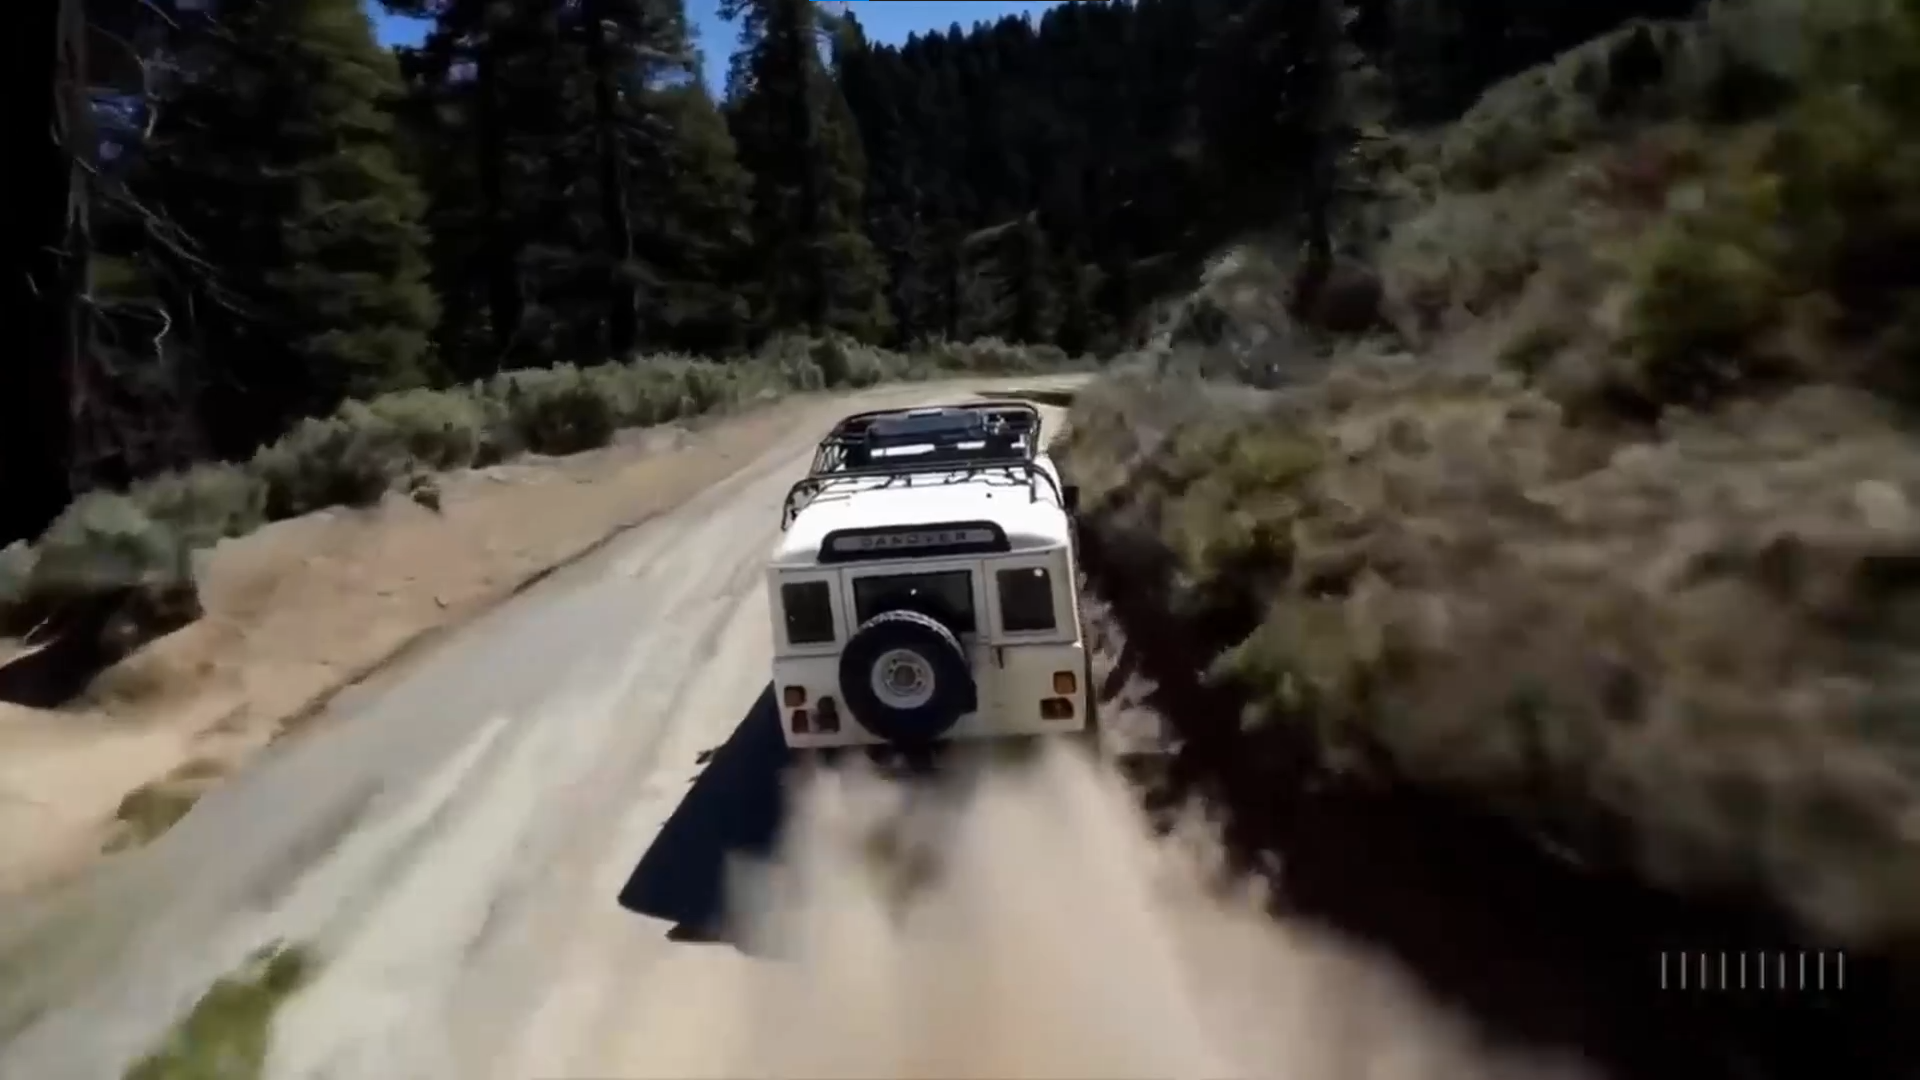
\includegraphics[width=0.8\textwidth]{videos/sora5-img.png}}{videos/sora5.mp4}
            \end{center}
        \end{column}
    \end{columns}

    \begin{columns}[T] % align columns
        \begin{column}{.33\textwidth}
            \begin{center}
                % \includemovie[autostart,loop,poster]{0.8\textwidth}{0.7\textheight}{sora3.mp4}
                \movie[externalviewer]{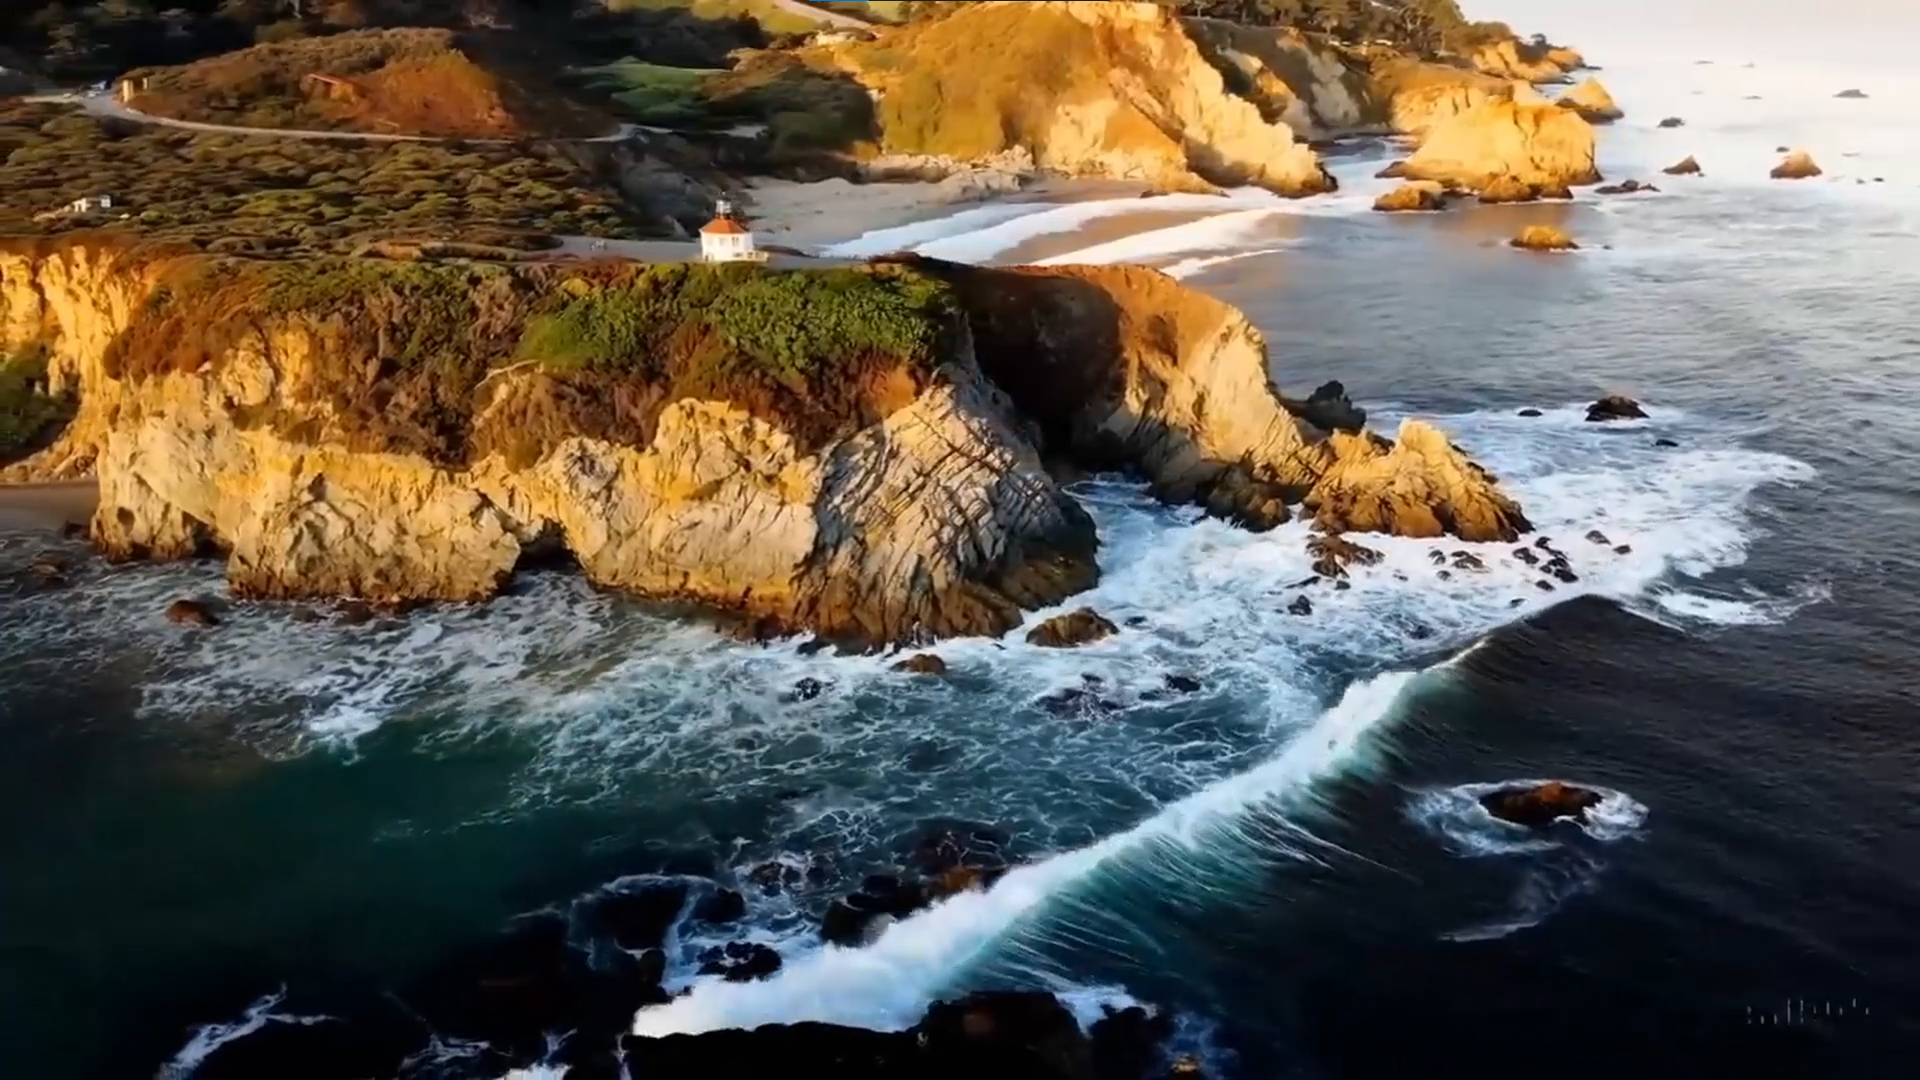
\includegraphics[width=0.8\textwidth]{videos/sora3-img.png}}{videos/sora3.mp4}
            \end{center}
        \end{column}%
        \begin{column}{.33\textwidth}
            \begin{center}
                % \includemovie[autostart,loop,poster]{0.8\textwidth}{0.7\textheight}{sora4.mp4}
                \movie[externalviewer]{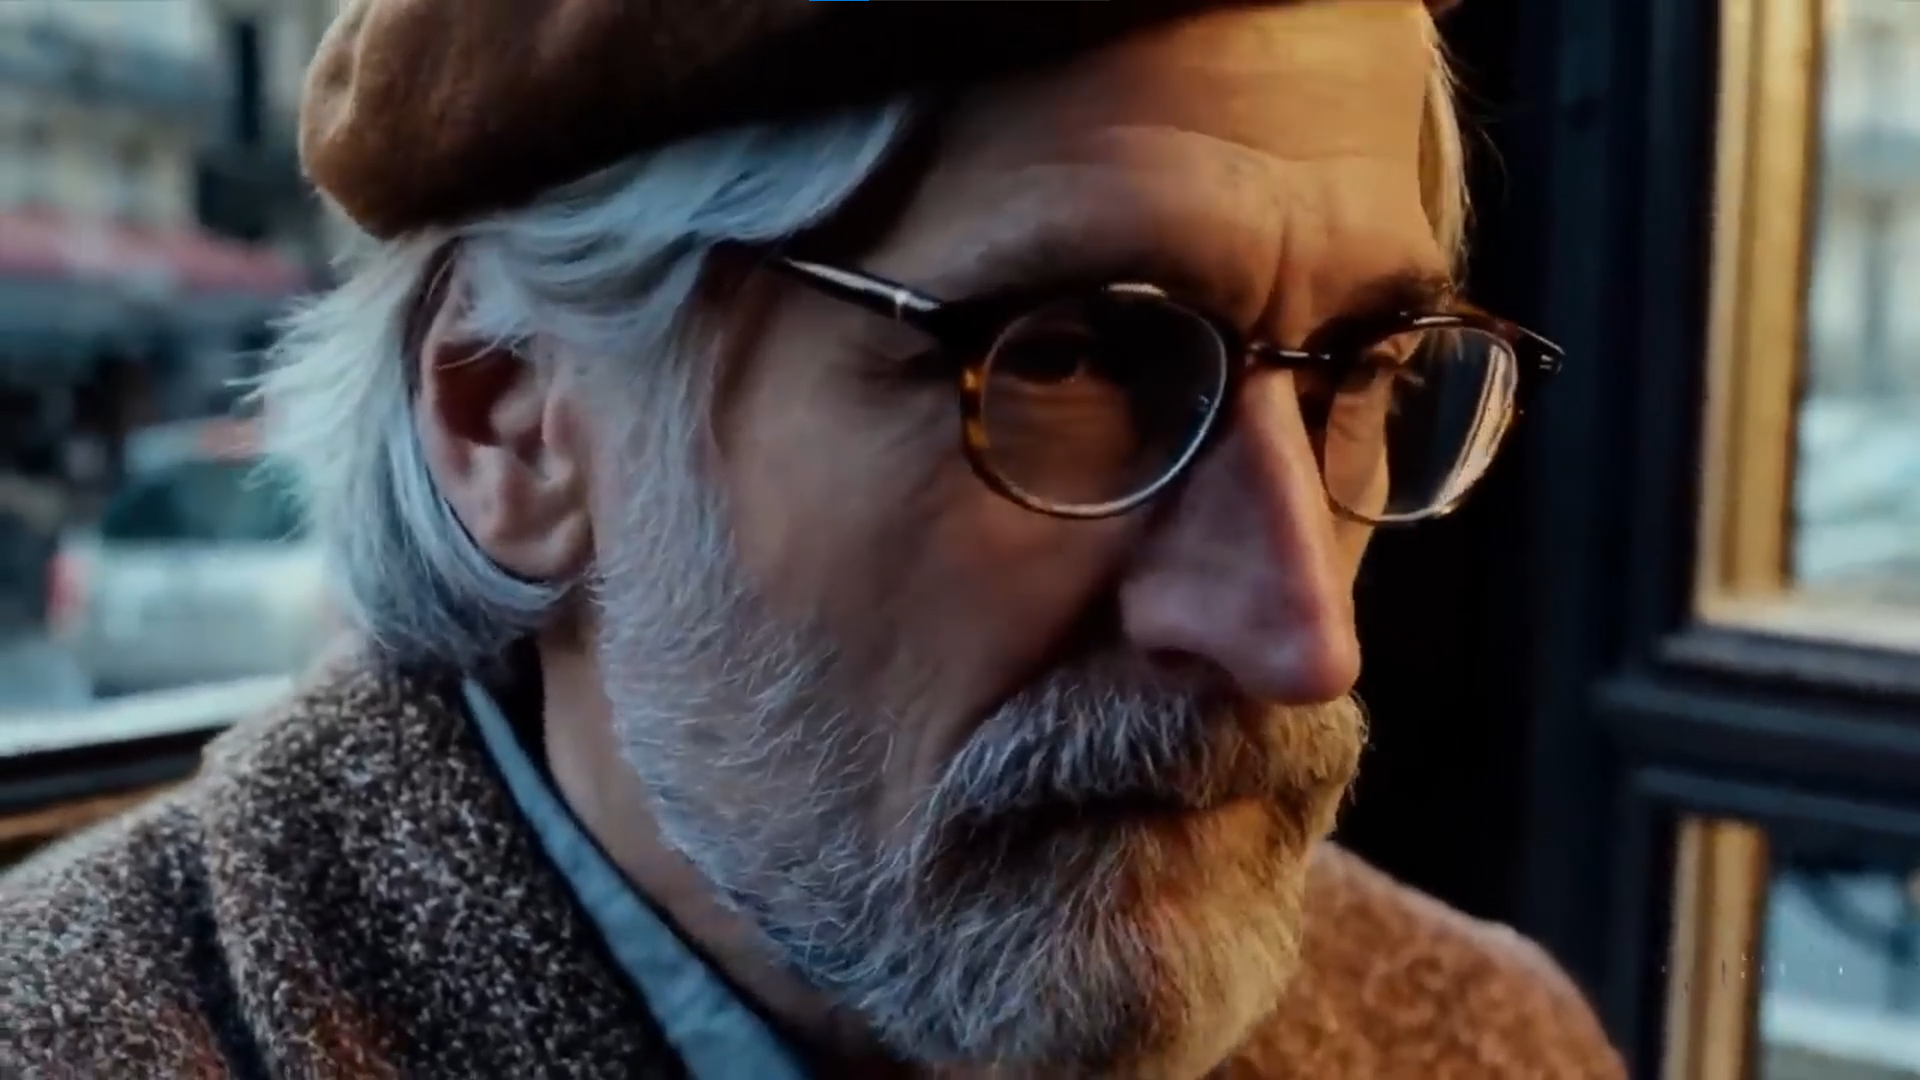
\includegraphics[width=0.8\textwidth]{videos/sora4-img.png}}{videos/sora4.mp4}
            \end{center}
        \end{column}%
        \begin{column}{.33\textwidth}
            \begin{center}
                % \includemovie[autostart,loop,poster]{0.8\textwidth}{0.7\textheight}{sora6.mp4}
                \movie[externalviewer]{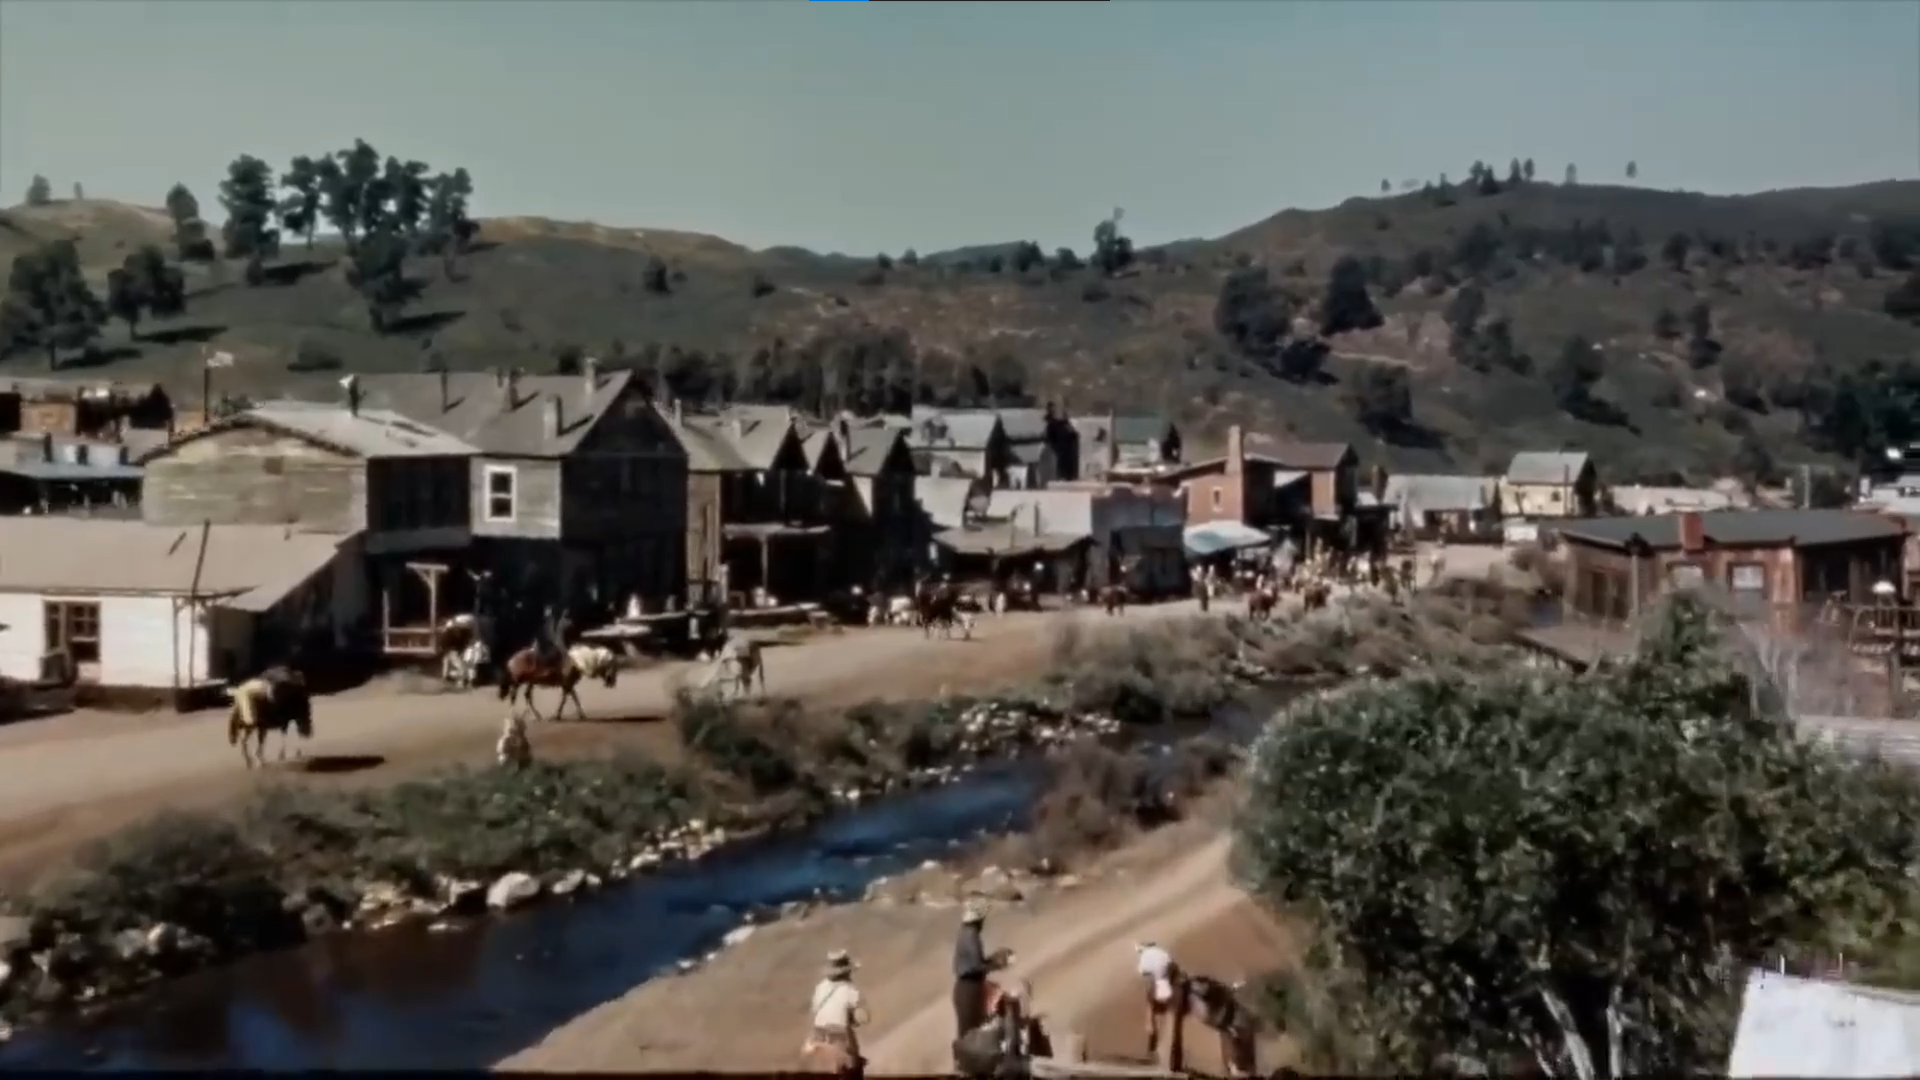
\includegraphics[width=0.8\textwidth]{videos/sora6-img.png}}{videos/sora6.mp4}
            \end{center}
        \end{column}
    \end{columns}
\end{frame}

\begin{frame}{Applicazioni al linguaggio}
    \begin{itemize}
    \item Modelli per la generazione di testo come \href{https://openai.com/index/gpt-4/}{GPT-4} \adjustbox{valign=m}{
\includegraphics[width=1.5cm]{logos/logo-chat-gpt4.png}} o \href{https://github.com/features/copilot}{Copilot} \adjustbox{valign=m}{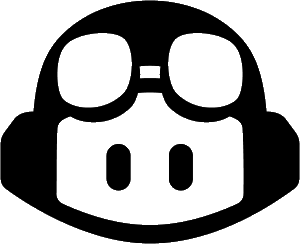
\includegraphics[width=0.5cm]{logos/logo-copilot.png}}.
    \item Esistono modelli open-source come \href{https://llama.meta.com/}{LLaMA-3} \adjustbox{valign=m}{
\includegraphics[width=1.5cm]{logos/logo-llama.png}} scaricabile graatuitamente dal loro sito. 
    \item Potete trovare modelli pre-addestrati e datasets su \href{https://huggingface.co/}{Hugging Face} \adjustbox{valign=m}{
\includegraphics[width=0.5cm]{logos/logo-hugging-face.png}} oppure su \href{https://www.kaggle.com/}{kaggle} \adjustbox{valign=m}{
\includegraphics[width=0.5cm]{logos/logo-kaggle.png}}.
\end{itemize}
    \pause
    \vspace{0.3cm}
    Per allenare Chat-GPT3, formata da $175$ miliardi di parametri, hanno impiegato $1023$ Nvidia A$100$ per $34$ giorni spendendo $5$ milioni di dollari in corrente.
    
    \vspace{0.3cm}
    \pause
    Anche per scaricare il modello più piccolo di LLaMA $3$ $8B$ sono necessari $20$ GB di VRAM e per il modello $LLaMA$ $3$ $70B$ sono necessari $140GB$ di spazio e $160GB$ di VRAM in $FP16$.
\end{frame}

\backmatter

\end{document}

To begin a  new line with some fixed vertical space
\vspace{\baselineskip}

\begin{block}{title}
\end{block}


% \begin{verbatim}  This begins a verbatim environment where the text is displayed exactly as it is written. This is useful for showing code snippets


% \begin{itemize}[<+->]  This starts an itemized (bulleted) list. The [<+->] option specifies that each item in the list should be revealed one by one as the presentation progresses (incrementally).


% \begin{frame}[fragile]{Writing a Simple Slide}  This starts a new slide (frame) titled "Writing a Simple Slide". The fragile option is used because the frame will contain verbatim text, which needs special handling in Beamer.


\uncover<2->{ <content> }  this means that the `content` is veasible from the second transition of the slide
The \uncover command makes the text visible starting from the specified slide number.


\begin{columns} % adding [onlytextwidth] the left margins will be set correctly
    \begin{column}{0.50\textwidth}
        
    \end{column}%
    \begin{column}{0.50\textwidth}
        
    \end{column}
\end{columns}


\textcolor{<color name>}{text}, \emph{}, \alert{} --> commands to brings the attention somewhere


% for a single monocrome block
\begin{themedColorBlock}{ `title` }
    `content`
\end{themedColorBlock}


% for block with highlighted title
\begin{themedTitleBlock}{ `title` }
    `content`
\end{themedTitleBlock}


% implemented styles for block's color
\themecolor{Black&White}, \themecolor{Red}, \themecolor{Yellow}, \themecolor{GreeenBrown}, 
\themecolor{DarkBlue}, \themecolor{Orange}, \themecolor{BlueGreen}, \themecolor{Green}, \themecolor{Blue}